%% Define the document style. The thesis stylesheet inherits from 'report'. 
%% I had once made a version inheriting from book. However the two versions are almost 
%% compatible. The main difference is that the other version supported 'parts'.
%% (extended from book) and this does not.
%% IST requires the thesis to be written in Arial or similar. Two arguments allow you 
%% to define the thesis font: 'Helvetica' and 'AvantGarde', which transforms normal font
%% into Helvetica or AvantGarde, respectively... dahhhh!
\documentclass[defaultstyle,10pt,master,Helvetica]{thesis}
%\documentclass[defaultstyle,12pt,phd]{thesis}
 
 
%% STYLESHEET SPECIFIC EXTRA COMMANDS (defined in thesis.cls):
%% ------------------------------------------------------------
%% \fancychapter{chaptername) -> Prints a fancier chapter
%% \hline{width} -> use for a replacement of the \hline command
%% \Mark1, \Mark2, \Mark3, ...

%% Defines an additional alphabet... not required in most cases
%% ------------------------------------------------------------
% \DeclareMathAlphabet{\mathpzc}{OT1}{pzc}{m}{it}

%% PACKAGE babel:
%% ---------------
%% The 'babel' package may correct some hyphenisation issues of latex. 
%% However in most situations it is not required.
% \usepackage[english]{babel}

%% PORTUGUESE WRITTEN DOCUMENTS
%% ---------------
%% If you are writting the document in portuguese you will have to use the following 
%% packages and commands:
% \usepackage[portuges]{babel} 
% \usepackage[fixlanguage]{babelbib}
% \selectbiblanguage{portuges}
% \def\chapterautorefname{Capítulo}
% \def\sectionautorefname{Sec\c{c}\~ao}
% \def\subsectionautorefname{Subsec\c{c}\~ao}
% \def\figureautorefname{Figura}
% \def\tableautorefname{Tabela}

%% SPECIAL LATIN CHARACTERS
%% ---------------
%% During the writting of the document you are likely to have to write some latin 
%% specific characters which are not typically available in english, e.g., vowels 
%% with accents. By default LaTeX2E is not prepared to handle these special characters. 
%% You can however add a package to handle these cases:
%%
%% if you are under linux, using UTF8 encoded characters, apply the following:
\usepackage[utf8]{inputenc}
%% if you are under windows, you will likely require the following package:
%\usepackage[latin1]{inputenc}

%% PACKAGE fontenc:
%% -----------------
%% chooses T1-fonts and allows correct automatic hyphenation.
%\usepackage[T1]{fontenc}

%% PACKAGE latexsym:
%% -----------------
%% Defines additional latex symbols. May be required for thesis with many math symbols.
%\usepackage{latexsym}

%% PACKAGE amsmath, amsthm, amssymb, amsfonts:
%% -------------------------------------------
%% This package is typically required. Among many other things it adds the possibility
%% to put symbols in bold by using \boldsymbol (not \mathbf); defines additional 
%% fonts and symbols; adds the \eqref command for citing equations. I prefer the style
%% "(x.xx)" for referering to an equation than to use "equation x.xx".
\usepackage{amsmath, amsthm, amssymb, amsfonts}

%% PACKAGE multirow, colortbl, longtable:
%% ---------------------------------------
%% These packages are most usefull for advanced tables. The first allows to join rows 
%% throuhg the command \multirow which works similarly with the command \multicolumn
%% The second package allows to color the table (both foreground and background)
%% The third package is only required when tables extend beyond the length of one page;
%% which typically does not happen and should be avoided
\usepackage{multirow}
\usepackage{colortbl}
% \usepackage{longtable}

%% PACKAGE graphics, epsfig, subfigure, caption:
%% ---------------------------------------------
%% Packages for figures... well you will certainly need these packages, with the exception
%% of the 'caption' package. This only allows to define extra caption options.
%% Notice that subfigure allows to place figures within figures with its own caption. It
%% should be avoided to create an eps file with subfigures. That will mean that you won't be 
%% able to reference those subfigures. Instead create an EPS file (the only graphics format supported
%% by latex) for each of the subfigures and then use the command \subfigure (see below).
\usepackage{graphics}
\usepackage{epsfig}
\usepackage{epstopdf}
\usepackage[hang,small,bf]{subfigure}
\usepackage{mathtools}
\usepackage{float}
\usepackage[export]{adjustbox}
\usepackage{setspace}
% \usepackage[hang,small,bf]{caption}

%% PACKAGE algorithmic, algorithm
%% ------------------------------
%% These packages are required if you need to describe an algorithm.
% \usepackage{algorithmic}
% \usepackage[chapter]{algorithm}

%% PACKAGE natbib/cite
%% -------------------
%% The two packages are not compatible, and you should use one of the two. Notice however that the
%% IEEE BiBTeX stylesheet is imcompatible with the natbib package. If using the IEEE format, use the 
%% cite package instead
%%
%% For numeric citations use:
\usepackage[square,numbers,sort&compress]{natbib}
%% For numeric author-year use:
% \usepackage[round,authoryear]{natbib}
%% For the cite package instead use:
%\usepackage{cite}

%% PACKAGE acronyum
%% -----------------
%% This package is most usefull for acronyms. The package garantees that all acronyms definitions are 
%% given at the first usage. IMPORTANT: do not use acronyms in titles/captions; otherwise the definition 
%% will appear on the table of contents.
\usepackage{acronym}

%% PACKAGE hyperref
%% -----------------
%% Set links for references and citations in document
%% Some MiKTeX distributions have faulty PDF creators in which case this package will not work correctly
%% Long live Linux :D
\usepackage[bookmarks=true]{hyperref}
\hypersetup{ colorlinks=false,
             citecolor=red,
             breaklinks=true,
             bookmarksnumbered=true,
             bookmarksopen=true,
             pdftitle={Multiple UDP ports for FaceWorks, a networked IP core used for debug},                 % EDIT THIS LINE
             pdfauthor={João Fernandes},                    % EDIT THIS LINE
             pdfsubject={Multiple UDP ports for FaceWorks},                  % EDIT THIS LINE
             pdfcreator={João Fernandes}, % EDIT THIS LINE
             pdfkeywords={}                             % EDIT THIS LINE
}

%% Set paragraph counter to alphanumeric mode
\renewcommand{\theparagraph}{\Alph{paragraph}~--}

%% Page formatting... It was correct for my master thesis... not sure it is still correct
%% edit as necessary
\hoffset 0in
\voffset 0in
\oddsidemargin 0.71cm
\evensidemargin 0.04cm
\marginparsep 0in
\topmargin -0.25cm
\textwidth 15cm
\textheight 23.5cm

\usepackage{fancyhdr}
\pagestyle{fancy}
\renewcommand{\chaptermark}[1]{\markboth{\thechapter.\ #1}{}}
\renewcommand{\sectionmark}[1]{\markright{\thesection\ #1}}
\fancyhf{} \fancyhead[LE]{\bfseries\nouppercase{\leftmark}}
\fancyhead[RO]{\bfseries\nouppercase{\rightmark}}
\fancyfoot[LE,RO]{\bfseries\thepage}
\renewcommand{\headrulewidth}{0.5pt}
\renewcommand{\footrulewidth}{0.5pt}
\addtolength{\headheight}{2pt} % make space for the rule
\fancypagestyle{plain}{%
   \fancyhead{} % get rid of headers
   \renewcommand{\headrulewidth}{0pt} % and the line
   \renewcommand{\footrulewidth}{0pt}
}
\fancypagestyle{blank}{%
   \fancyhf{} % get rid of headers and footers
   \renewcommand{\headrulewidth}{0pt} % and the line
   \renewcommand{\footrulewidth}{0pt}
}
\fancypagestyle{abstract}{%
   \fancyhead{}
   \renewcommand{\headrulewidth}{0pt}
   \renewcommand{\footrulewidth}{0.5pt}
}
\fancypagestyle{document}{%
	\fancyhf{} \fancyhead[LE]{\bfseries\nouppercase{\leftmark}}
	\fancyhead[RO]{\bfseries\nouppercase{\rightmark}}
	\fancyfoot[LE,RO]{\bfseries\thepage}
	\renewcommand{\headrulewidth}{0.5pt}
	\renewcommand{\footrulewidth}{0.5pt}
	\addtolength{\headheight}{2pt} % make space for the rule
}
\setcounter{secnumdepth} {5}
\setcounter{tocdepth} {5}
\renewcommand{\thesubsubsection}{\thesubsection.\Alph{subsubsection}}

\renewcommand{\subfigtopskip}{0.3 cm}
\renewcommand{\subfigbottomskip}{0.2 cm}
\renewcommand{\subfigcapskip}{0.3 cm}
\renewcommand{\subfigcapmargin}{0.2 cm}


\begin{document}

% Add PDF bookmark 
\pdfbookmark[0]{Multiple UDP ports for FaceWorks}{Title}

%%%%%%%%%%%%%%%%%%%%%%%%%%%%%%%%%%%%%%%%%%%%%%%%%%%%%%%%%%%%%%%%%%%%%%%%%%%%%%%%%%%%%%%%%%%%%%%%
% DEFINE THE TITLEPAGE
% remember that IST requires for the titlepage to be written in portuguese
%%%%%%%%%%%%%%%%%%%%%%%%%%%%%%%%%%%%%%%%%%%%%%%%%%%%%%%%%%%%%%%%%%%%%%%%%%%%%%%%%%%%%%%%%%%%%%%%
% REQUIRED:
% The university logo image: first and second arguments are the (top,left) position of the logo. 
% IST rules force it to be 2cm
\univlogo{2cm}{1cm}{IST_A_CMYK_POS.eps} %%{logo_ist_web.eps}
% OPTIONAL:
% The thesis logo image: first and second arguments are the position of the logo. 
%\thesislogo{2.5cm}{6cm}{thesis_logo.eps}

% Thesis title
\title{Multiple UDP ports for FaceWorks, a networked IP core used for debug}

% Author and highest current degree (not the one you are applying to)
\author{João Carlos dos Santos Fernandes}
\degree{Electrical and Computer Engineering}
% This is not on the new IST MSc stylesheet... however for PhD dissertations it will most likely be required
%\otherdegree{Mestre}

% The supervisor. Use the second command if required.
% Always remember that 'Professor' should only be used for a supervisor with a Cathedra
% -- not in Portugal
\supervisor{Prof. José João Henriques Teixeira de Sousa}
%\othersupervisor{Engenheiro Ricardo Jorge Santos Martins}

% Date of the dissertation
\date{November 2013}

% Is this the final version? Place false when delivering the first part.
% The juri members will not be printed in that case. Place true after the juri has accepted the thesis
\finalthesis{true}

% The members of the Juri
% Always remember that 'Professor' should only be used for a juri member with a Cathedra
\presidentofjury{Prof. João Manuel Torres Caldinhas Simões Vaz}
\vogalone{Prof. Paulo Ferreira Godinho Flores}
%\vogaltwo{Doutor whatever full name 3}
% \vogalthree{Doutor whatever full name 4}
% \vogalfour{Doutor whatever full name 5}
%%%%%%%%%%%%%%%%%%%%%%%%%%%%%%%%%%%%%%%%%%%%%%%%%%%%%%%%%%%%%%%%%%%%%%%%%%%%%%%%%%%%%%%%%%%%%%%%

% print titlepage
\maketitle
%\clearpage

% Since I am using double sided pages, the second page should be white.
% Remember that when delivering the dissertation, IST requires for the cover to appear twice.
\thispagestyle{empty}
\cleardoublepage

\setcounter{page}{1} \pagenumbering{roman}

\baselineskip 18pt % line spacing: -12pt for single spacing
                   %               -18pt for 1 1/2 spacing
                   %               -24pt for double spacing

%\pdfbookmark{Acknowledgments}{Acknowledgments}
%\begin{acknowledgments}
%Thanks to the author of this document... If you are not thanking than... you are not %thanking!!!
%\end{acknowledgments}

%\pdfbookmark{Abstract}{Abstract}

\begin{abstract}
\addcontentsline{toc}{chapter}{Abstract}
This thesis presents an implementation of multiple \ac{UDP} ports for FaceWorks, an \ac{ILP} core used for hardware test and debug over the \ac{UDP}/\acs{IP} network protocol, which is a patented and proprietary technology of the company Coreworks SA. The objective of having multiple ports is to allow multiple software processes to independently control the device under test (eg. multiple audio streams driven by multiple programs). An overview of the FaceWorks technology and its possible applications is presented, with emphasis on the \ac{CWDP}, which was added on top of the common \ac{UDP} protocol to enable test and debug functions. The FaceWorks hardware has been converted to Verilog, upgraded to support two \ac{UDP} ports, and tested using the Verilator simulator and an \ac{FPGA} board. A SystemC model of the core is automatically generated and simulated by Verilator. A SystemC testbench that uses network sockets has been written to fully replicate the hardware behavior in simulation. A PC software driver and an application which connects to the two \ac{UDP} ports for testing the system have been developed. This application connects to both the SystemC model or \ac{FPGA} board, indistinguishably. Experiments and implementation results are reported.

\end{abstract}

\begin{keywords}
Ethernet, UDP, CWDP, System-on-Chip, Verilator, Verification
\end{keywords}
\clearpage
\thispagestyle{empty}
\cleardoublepage

%\pdfbookmark{Resumo}{Resumo}

\begin{resumo}
\addcontentsline{toc}{chapter}{Resumo}
Esta tese apresenta uma implementação de portas \ac{UDP} múltiplas para o FaceWorks, um núcleo de Propriedade Intelectual utilizado para o teste  e depuração de \textit{hardware}. Funciona sobre o protocolo de rede \ac{UDP}/\ac{IP}, e é uma tecnologia patenteada e propriedade da empresa Coreworks SA. O objectivo das portas múltiplas é permitir que vários processos de \textit{software} possam controlar de forma independente o dispositivo de teste (múltiplos fluxos de áudio gerados por vários programas). Uma descrição geral da tecnologia FaceWorks e suas possíveis aplicações é apresentada, dando ênfase ao \textit{\acf{CWDP}}, que consiste numa camada adicionada sobre o protocolo \ac{UDP} para realizar as funções de teste e depuração. A descrição do FaceWorks foi convertida para Verilog, actualizada para suportar duas portas \ac{UDP}, e testada utilizando o simulador Verilator e uma placa de \ac{FPGA}. 
Foi gerado automaticamente um modelo SystemC do núcleo e simulado com recurso ao Verilator.
Foi descrita uma bancada de teste em SystemC que usa \textit{sockets} de rede para replicar totalmente o comportamento do \textit{hardware} em simulação. Foram desenvolvidos um controlador de software para PC e uma aplicação que se liga às duas portas \ac{UDP} para testar o sistema. A aplicação desenvolvida interage indiferentemente com o modelo SystemC ou com a placa de \ac{FPGA}. Experiências e resultados de implementação são apresentados.
\end{resumo}

\begin{palavraschave}
Ethernet, UDP, CWDP, Sistema-num-Chip, Verilator, Verificação
\end{palavraschave}

\clearpage
\thispagestyle{empty}
\cleardoublepage

% This is required for the fancy chapters
%\dominitoc
%\dominilof
%\dominilot
%\dominiloac
%%%%%%%%%%%%%%%%%%%%%%%%%%%%%%%%%%%%%%%%%%%%%%%%%%%%%%%%%%%%%%%%%%%%%%
% List of contents
%\renewcommand{\baselinestretch}{1}
%\pdfbookmark[0]{Index}{index}
%\pdfbookmark[1]{Contents}{toc}
\addcontentsline{toc}{chapter}{Contents}
\tableofcontents
% \contentsline{chapter}{References}{\pageref{bib}}
\cleardoublepage
%\renewcommand{\baselinestretch}{1.5}

%%%%%%%%%%%%%%%%%%%%%%%%%%%%%%%%%%%%%%%%%%%%%%%%%%%%%%%%%%%%%%%%%%%%%%
% List of figures
%\pdfbookmark[1]{List of Figures}{lof}
\addcontentsline{toc}{chapter}{List of Figures}
\listoffigures
\cleardoublepage

%%%%%%%%%%%%%%%%%%%%%%%%%%%%%%%%%%%%%%%%%%%%%%%%%%%%%%%%%%%%%%%%%%%%%%
% List of tables
%\pdfbookmark[1]{List of Tables}{lot}
\addcontentsline{toc}{chapter}{List of Tables}
\listoftables
\cleardoublepage

% %%%%%%%%%%%%%%%%%%%%%%%%%%%%%%%%%%%%%%%%%%%%%%%%%%%%%%%%%%%%%%%%%%%%%%
% % List of algorithms
% Requires packages algorithmic, algorithm
% \pdfbookmark[1]{List of Algorithms}{loa}
% \listofalgorithms
% \cleardoublepage


% %%%%%%%%%%%%%%%%%%%%%%%%%%%%%%%%%%%%%%%%%%%%%%%%%%%%%%%%%%%%%%%%%%%%%%
% % List of acronyms
%\pdfbookmark[1]{List of Acronyms}{List of Acronyms}
%\chapter*{List of Acronyms}
\vspace*{1.95cm} \hspace*{-0.5cm} %,88
\textbf{{\huge \sffamily List of Acronyms}\\}
\vspace*{0.5cm}
\begin{acronym}
\addcontentsline{toc}{chapter}{List of Acronyms}
\thispagestyle{plain}
\setcounter{page}{13}
\acro{ACK}{Acknowledge}
\acro{ARP}{Address Resolution Protocol}
\acro{BRAM}{Block Random Access Memory}
\acro{CRC}{Cyclic Redundancy Check}
\acro{CWDP}{Coreworks Datagram Protocol}
\acro{DCM}{Digital Clock Manager}
\acro{DPLL}{Digital Phase-Locked Loop}
\acro{FIFO}{First In First Out}
\acro{FPGA}{Field Programmable Logic Array}
\acro{FCS}{Frame Check Sequence}
\acro{FSM}{Finite State Machine}
\acro{GPU}{Graphics Processing Unit}
\acro{HDL}{Hardware Description Language}
\acro{IFG}{inter-frame gap}
\acro{ILA}{Integrated logic analyzer}
\acro{ILP}[IP]{Intelectual Property}
\acro{IP}[IP]{Internet Protocol}
\acro{IO}{Input-Output}
\acro{LAN}{Local Area Network}
\acro{LSB}{Less Significant Bit}
\thispagestyle{plain}
\acro{MAC}{Media Access Control}
\thispagestyle{plain}
\acro{MII}{Media Independent Interface}
\thispagestyle{plain}
\acro{MSB}{Most Significant Bit}
\acro{MTU}{Maximum Transmission Unit}
\acro{NACK}{Not acknowledge}
\acro{OS}{Operating System}
\acro{OSI}{Open Systems Interconnection}
\acro{OWD}{One Way Delay}
\acro{PC}{Personal Computer}
\acro{PHY}{Ethernet Physical Transceiver}
\acro{PLL}{Phase-Locked Loop}
\acro{RAM}{Random Access Memory}
\acro{RTT}{Round-Trip delay Time}
\acro{RHS}{Right Hand Side}
\acro{SFD}{Start Frame Delimiter}
\acro{SoC}{System-on-Chip}
\acro{TCP}{Transmission Control Protocol}
\acro{UDP}{User Datagram Protocol}
\acro{VHDL}{VHSIC Hardware Description Language}
\acro{XST}{Xilinx Synthesis Tool}
\end{acronym}

\cleardoublepage

% Pages number is starting now with arabic style... until now it was on roman mode
\setcounter{page}{1} \pagenumbering{arabic}
\baselineskip 18pt

% %%%%%%%%%%%%%%%%%%%%%%%%%%%%%%%%%%%%%%%%%%%%%%%%%%%%%%%%%%%%%%%%%%%%%%
% The Introduction:
% %%%%%%%%%%%%%%%%%%%%%%%%%%%%%%%%%%%%%%%%%%%%%%%%%%%%%%%%%%%%%%%%%%%%%%
% Notice that I am using my own chapter style, instead of the default one
\fancychapter{Introduction}
\acresetall

In this chapter the scope of the work is presented, the problem addressed is formulated, the proposed solution is explained, the objectives of the work are stated, and the thesis contents is outlined.


\section{Scope}

Nowadays, integrated circuit designers are presented with extremely short design cycles. To deliver on time, companies are required to optimize the design flow. Of the many solutions created, one of the most successful is the reuse of pre-existent and complex blocks, often called Intellectual Property Cores, or simply \acs{ILP} Cores.

A core with well defined and specialized functionality is easier to implement and verify, and can be reused later in other designs. This greatly overcomes some of the complexity of the design and verification process.

Out of this idea a brand new business model has flourished, where \acs{ILP} providers produce verified hardware \acs{ILP} libraries, sometimes associated with software \acs{ILP} libraries, and \acs{ILP} integrators select and integrate multiple \acs{ILP} cores from different vendors on a \ac{SoC}.

Due to the consistent evolution of semiconductor manufacturing processes, integrated circuit manufacturers are raising the gate count per die area year after year, and lowering other metrics such as power consumption and cost per gate \cite[p. 24]{XilinxConsump}. Table \ref{table:Table Transistor Densisty} shows the complexity of some large devices from various manufacturers in terms of their transistor area density.

The latest developments in \acfp{FPGA}, placed high-end \acsp{FPGA} as one of the devices with the highest transistor counts per die area. Launched in September 2011 by Xilinx, the Virtex-7 2000-T presented an astonishing value of 12.85 million transistors per square mm. This is more than the generation of \acp{GPU} launched later by NVIDIA, in April 2012, the GTX 670 (Kepler), with 12.04 million transistors per square mm. Both devices are fabricated using 28nm technology.



With such high transistor density, several \ac{FPGA} devices, from mid to high-end, already integrate up to 2 million logic cells and hard blocks for functions like DSP, PCI-E controllers, Ethernet \acp{MAC}, memory controllers, DCM/PLL, BRAMs, etc. These highly heterogeneous devices allow engineers not only to use \acp{FPGA} as a prototyping platform but also as the target platform.

As \acp{FPGA} present themselves as flexible and cost effective platforms to test, verify and produce \acs{ILP} cores, challenges arise on how to properly communicate independently with each \acs{ILP} core in the \ac{FPGA}. \acs{ILP} cores need to be observed, configured, tested and debugged. Complex hardware systems demand complicated and concurrent testing and debug methods, often requiring expensive equipment to be used.
\clearpage
\newcommand{\greyrow}{\rowcolor[rgb]{0.9,0.9,0.9}}
\newcommand{\whiterow}{\rowcolor[rgb]{1,1,1}}
\newcommand{\greycell}[1]{\multicolumn{1}{{>{\columncolor[rgb]{0.9,0.9,0.9}}c}}{#1}}
\newcommand{\lightgreycell}[1]{\multicolumn{1}{{>{\columncolor[rgb]{0.9,0.9,0.9}}c}}{#1}}
\newcommand{\mediumgreycell}[1]{\multicolumn{1}{{>{\columncolor[rgb]{0.8,0.8,0.8}}c}}{#1}}
\newcommand{\darkgreycell}[1]{\multicolumn{1}{{>{\columncolor[rgb]{0.7,0.7,0.7}}c}}{#1}}
\newcommand{\whitecell}[1]{\multicolumn{1}{{>{\columncolor[rgb]{1,1,1}}c}}{#1}}

\newcommand{\cellformatG}[1]{\multicolumn{1}{{>{\columncolor[rgb]{.9,.9,.9}}c}}{#1}}
\newcommand{\cellformatW}[1]{\multicolumn{1}{{>{\columncolor[rgb]{1,1,1}}c}}{#1}}
\newcommand{\cellformatlG}[1]{\multicolumn{1}{{|>{\columncolor[rgb]{.9,.9,.9}}c}}{#1}}
\newcommand{\cellformatlW}[1]{\multicolumn{1}{{|>{\columncolor[rgb]{1,1,1}}c}}{#1}}
\newcommand{\cellformatrG}[1]{\multicolumn{1}{{>{\columncolor[rgb]{.9,.9,.9}}c|}}{#1}}
\newcommand{\cellformatrW}[1]{\multicolumn{1}{{>{\columncolor[rgb]{1,1,1}}c|}}{#1}}
\newcommand{\cellformatlrG}[1]{\multicolumn{1}{{|>{\columncolor[rgb]{.9,.9,.9}}c|}}{#1}}
\newcommand{\cellformatlrW}[1]{\multicolumn{1}{{|>{\columncolor[rgb]{1,1,1}}c|}}{#1}}

\begin{table}[h]
\centering
\caption{Transistor Density Comparison}
\label{table:Table Transistor Densisty}
\begin{tabular}{c c c c}
\hlinew{0.08cm}
\cellformatrG{}&\cellformatlrG{}&\cellformatlrG{}&\cellformatlG{}\\
\cellformatrG{\multirow{-2}{*}{Device}} &
\cellformatlrG{\multirow{-2}{2cm}{\centering Millions of Transistors}}&
\cellformatlrG{\multirow{-2}{1.8cm}{\centering Die Area $(mm^2)$ }}&
\cellformatlG{\multirow{-2}{2cm}{\centering Density}}
\\
\hlinew{0.08cm}
\greyrow \multicolumn{4}{c}{GPU}
\\
\hlinew{0.04cm}
\cellformatrW{Nvidia GTX 670 (2012 - 28 nm) \cite{G600Wiki2013} } & \cellformatlrW{3540} & \cellformatlrW{294} & \cellformatlW{\emph{12.04}}\\
\cellformatrW{AMD Tahit RV1070 (2011 - 28nm) \cite{CountWiki2013} } & \cellformatlrW{4312} & \cellformatlrW{365} & \cellformatlW{11.81}\\
\cellformatrW{Nvidia GF100 Fermi(2010 - 40 nm) \cite{CountWiki2013} } & \cellformatlrW{3200} & \cellformatlrW{526} & \cellformatlW{6.08}\\
\cellformatrW{AMD Caymn RV870 (2010 - 40 nm) \cite{CountWiki2013} } & \cellformatlrW{2154} & \cellformatlrW{334} & \cellformatlW{6.44}\\
\cellformatrW{AMD RV790XT (2008 - 55nm) \cite{CountWiki2013} } & \cellformatlrW{959} & \cellformatlrW{282} & \cellformatlW{3.40}\\
\cellformatrW{NVIDIA GT200 Tesla (2008 - 55nm) \cite{CountWiki2013} } & \cellformatlrW{1400} & \cellformatlrW{576} & \cellformatlW{2.43}\\
\hlinew{0.08cm}
\greyrow \multicolumn{4}{c}{CPU}
\\
\hlinew{0.04cm}
\cellformatrW{Intel Ivy Bridge (22 nm -2012) \cite{AnnandIvy2012}} & \cellformatlrW{1400} & \cellformatlrW{160} & \cellformatlW{8.75}\\
\cellformatrW{Amd Trinity (32nm - 2012) \cite{AnnandTrinity2012}} & \cellformatlrW{1178} & \cellformatlrW{228} & \cellformatlW{5.17}\\
\cellformatrW{Intel Xeon 2690EP (32 nm -2011) \cite{JohanXeon2011}} & \cellformatlrW{2260} & \cellformatlrW{416} & \cellformatlW{5.43}\\
\cellformatrW{Amd Bulldozer 8 Cores (32 nm - 2011) \cite{AnnandBulldozer2011} } & \cellformatlrW{1200} & \cellformatlrW{315} & \cellformatlW{3.81}\\
\multicolumn{4}{c}{\vspace*{-0.3cm}}\\
%%%%%%%%%%%%% Third PART OF THE TABLE %%%%%%%%%%%%%%%%%%%%%%%%
\hlinew{0.08cm}
\greyrow \multicolumn{4}{c}{FPGA}
\\
\hlinew{0.04cm}
\cellformatrW{Xilinx Virtex-7 2000 T (28nm - 2011) \cite{yannou2011X3d} } & \cellformatlrW{6800} & \cellformatlrW{529} & \cellformatlW{\emph12.85}\\
\end{tabular}
\end{table}

To solve this problem, the company Coreworks SA created and patented a technology \cite[US 2008/0288652]{ncapat}, \cite[EP 2003571/A2]{ncapateu} that uses a simple PC and the office network to exercise multiple cores in the \ac{FPGA}. The technology has been called Core Access Networks\textregistered and comprises the FaceWorks \acs{ILP} core, which is the gateway between the \acs{ILP} Cores under test and a software program (test driver) running on the PC. 

Prior devices for observation, configuration, testing and debugging on-chip cores resorted to already existing communication protocols. Most of them used low-speed serial protocols with low pin counts, such as I2C, SPI or JTAG, which was initially created to test printed circuit boards and later extended to chips.

FaceWorks implements the \ac{UDP}/\ac{IP}/Ethernet protocol stack in hardware, dispensing with an embedded processor and a software protocol stack. In addition, the \acf{CWDP} was created to implement test and debug functions on top of the \ac{UDP}/\ac{IP} stack. Other functions such as data streaming can also be performed with this technology. This solution represents an almost costless, high-speed and versatile test and debug mechanism.


\section{Problem}

The implementation of FaceWorks that existed when this work started used only a single \ac{UDP} port to communicate with the \ac{FPGA} board. The main problem of having a single port is that, to exercise \acs{ILP} modules concurrently, the test driver application becomes very difficult to write. This is the problem that this work solves.

\section{Solution}

To solve the problem formulated in the previous section, it has been decided to increase the number of \ac{UDP} ports supported by FaceWorks, in order to allow multiple software processes or threads to independently and concurrently stimulate and observe multiple \ac{ILP} cores in the system.


\section{Objectives}
The main objectives of this thesis are the following:
\begin{enumerate}

\item Upgrade the FaceWorks hardware so that it can support multiple and concurrent channels by means of multiple \ac{UDP} ports. The upgrade is done using the Verilog language, which implies converting the original code from \ac{VHDL} to Verilog.

\item Write a SystemC verification environment (testbench) that uses the FaceWorks SystemC model generated by the Verilator tool.

\item Write an application that generates and sends test patterns for the multiple \ac{UDP} ports, receives the responses and checks the results. This application can communicate indistinguishably with either the FPGA board or the SystemC testbench.

\end{enumerate}

\section{Outline}
This thesis is structured in the given form:
\begin{description}
\item[Chapter 2] \hfill \\ The main concepts of the protocols and interfaces used by FaceWorks are presented. The existing FaceWorks architecture is also presented.
\item[Chapter 3] \hfill \\ The development methodology for both the software and hardware components of this work is presented.
\item[Chapter 4] \hfill \\ The architecture of the application that uses Verilator to create a FaceWorks simulator is presented.
\item[Chapter 5] \hfill \\ Implementations results are presented and compared with the previous implementation. A caracterization of the network is performed and an analysis of the network performance of FaceWorks is presented.
\item[Chapter 6] \hfill \\ Conclusions are drawn. Future modifications and alternative implementations are discussed.

\end{description}
\cleardoublepage

% %%%%%%%%%%%%%%%%%%%%%%%%%%%%%%%%%%%%%%%%%%%%%%%%%%%%%%%%%%%%%%%%%%%%%%
% Your work: Chapter 6
% %%%%%%%%%%%%%%%%%%%%%%%%%%%%%%%%%%%%%%%%%%%%%%%%%%%%%%%%%%%%%%%%%%%%%%
\fancychapter{Background}

In this chapter the FaceWorks IP core is introduced, and its interfaces and protocols are explained. The existing FaceWorks architecture is shown in Figure \ref{fig:FW-diag}. In the following sections, the implementations of the \ac{MII} interface, data link, network and transport layers are presented.

\begin{figure}[h]
  \centering
      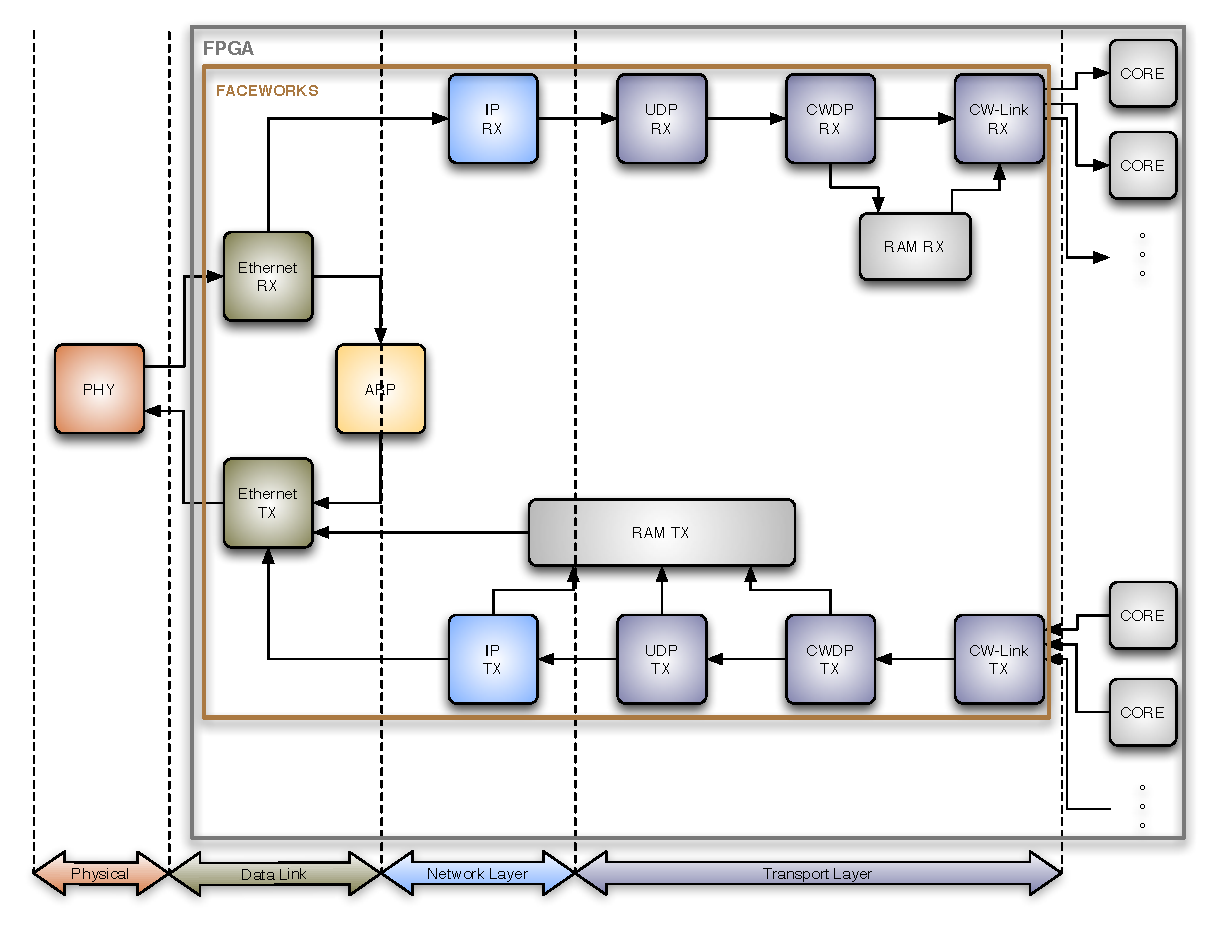
\includegraphics[scale=0.75,center]{Diagrams/FW.pdf}
  \caption{FaceWorks Block Diagram}\label{fig:FW-diag}
\end{figure}



\section{Media Independent Interface}

The \ac{MII}\cite{ieee802.3b} is a well known industry standard for the interface between the \ac{MAC} and the \ac{PHY}. In terms of the OSI layer model, it implements the interface between the physical layer and the data link layer. MII is used to interconnect the FaceWorks core in the \ac{FPGA} and the \ac{PHY} chip on the same board, as depicted in Figure \ref{fig:MII}. The MII signals of the FaceWorks core are presented in Table \ref{table:MII-Table}.

\begin{figure}[h]
  \centering
      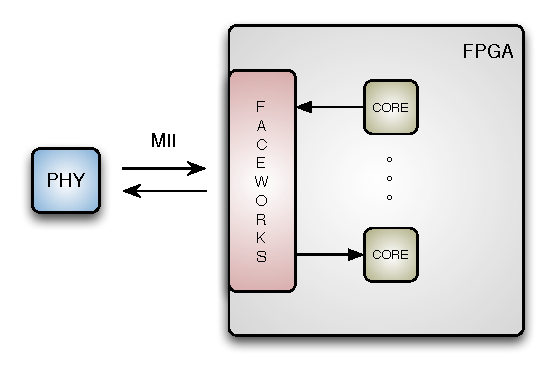
\includegraphics[scale=1.25,center]{Diagrams/MII.pdf}
  \caption{Interconnection of \ac{PHY} and FaceWorks using MII}\label{fig:MII}
\end{figure}

Both \texttt{TX\_CLK} and \texttt{RX\_CLK} are 25 MHZ clock signals, required for a \ac{PHY} operating at 100 Mbps. The signal \texttt{RX\_ER} is not used. Instead the \ac{CRC} field provided by the \ac{MAC} layer is used to check the frame content. The signal \texttt{mdio} is in high-impedance as both the managing signals are not used.

\begin{table}[h]
\centering
\caption{Media Independent Interface Signals}
\label{table:MII-Table}
\begin{tabular}{c c l}
\hlinew{0.08cm}
\cellformatrG{}&
\cellformatlrG{}&
\cellformatlG{}
\\
\cellformatrG{\multirow{-2}{2cm}{\centering Signals}} &
\cellformatlrG{\multirow{-2}{2cm}{\centering Direction}} &
\cellformatlG{\multirow{-2}{2cm}{\centering Description}}
\\
\hlinew{0.04cm}
\greyrow \multicolumn{3}{c}{Transmit}
\\
\hlinew{0.04cm}
\cellformatrW{ TX\_CLK }& 
\cellformatlrW{ input }&
Clock signal reference for the transmit signals
\\
\hlinew{0.04cm}
\cellformatrW{ TX\_EN }& 
\cellformatlrW{ output }&
MAC is presenting data on the MII for transmission
\\
\hlinew{0.04cm}
\cellformatrW{ TX\_D[3:0] }& 
\cellformatlrW{ output }&
Transmit Data
\\
\hlinew{0.04cm}
\cellformatrW{ TX\_ER }& 
\cellformatlrW{ output  }&
MAC Signals the transmission of a coding error on the frame
\\
%\multicolumn{3}{c}{\vspace*{-0.3cm}}\\
%%%%%%%%%%%%% SECOND PART OF THE TABLE %%%%%%%%%%%%%%%%%%%%%%%%
%\hlinew{0.08cm}
%\cellformatrG{}&
%\cellformatlrG{}&
%\cellformatlG{}
%\\
\hlinew{0.04cm}
\greyrow  \multicolumn{3}{c}{ Receive }\\
\hlinew{0.04cm}
\cellformatrW{ RX\_CLK }& 
\cellformatlrW{ input }&
Clock signal reference for the receive signals
\\
\hlinew{0.04cm}
\cellformatrW{ RX\_DV }& 
\cellformatlrW{ input}&
MII is presenting data to the MAC
\\
\hlinew{0.04cm}
\cellformatrW{ RX\_D[3:0] }& 
\cellformatlrW{ input }&
Receive Data
\\
\hlinew{0.04cm}
\cellformatrW{ RX\_ER }& 
\cellformatlrW{ input  }&
PHY signals the transmission of error on the frame
\\
%\multicolumn{3}{c}{\vspace*{-0.3cm}}\\
%%%%%%%%%%%%% Third PART OF THE TABLE %%%%%%%%%%%%%%%%%%%%%%%%
%\hlinew{0.08cm}
%\cellformatrG{}&
%\cellformatlrG{}&
%\cellformatlG{}
%\\
\hlinew{0.04cm}
\greyrow \multicolumn{3}{c}{Management }\\
\hlinew{0.04cm}
\cellformatrW{ MDC}& 
\cellformatlrW{ input }&
Management data clock
\\
\hlinew{0.04cm}
\cellformatrW{ MDIO}& 
\cellformatlrW{ output }&
Management data input/output
\end{tabular}
\end{table}



\clearpage
\subsection{Data Stream}

Packets transmitted through the \ac{MII}, are framed as shown in Figure \ref{fig:MII-frame}. Below follows an explanation of each field.

\begin{figure}[h]
  \centering
      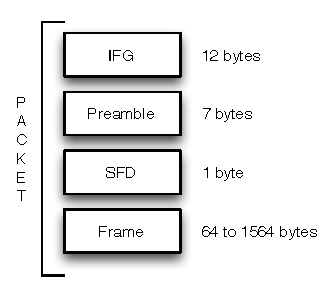
\includegraphics[scale=1.25,center]{Diagrams/MII-packet.pdf}
  \caption{\ac{MII} Packet}\label{fig:MII-frame}
\end{figure}

\paragraph*{IFG} The \ac{IFG} is a period of 12 bytes in which the \texttt{TX\_EN} or the \texttt{RX\_EN} signals are asserted low to produce an idle time between the previous packet and the current packet. This allows both the \ac{PHY} and the \ac{MAC} to process the previous packet, and prepare for the reception of the new packet.

\paragraph*{Preamble} The preamble consists of a sequence of 56 bits of alternating 1's and 0's \footnote{The stream is transmitted from left to right.}, in order to allow the receiver \ac{PHY} \ac{DPLL} to lock.

\paragraph*{SFD} The \ac{SFD} consists in the bit sequence 10101011 \footnotemark[\value{footnote}], marks the start of the packet and the end of the preamble.

\paragraph*{Frame} Contains the actual payload that is transmitted through the MII.

\section{Media Access Control}

The \acf{MAC}\cite{ieee802.3a} protocol together with the \ac{MII} interface implement the Ethernet data link layer and the interface to the physical layer, respectively.

From the packet format defined previously for the \ac{MII} interface, the \ac{MAC} encapsulates the data payload with a 14-byte header and a 4-byte \ac{CRC} trailer, as shown in Figure \ref{fig:Eth-frame}. Below follows an explanation of each field.

\begin{figure}[h]
  \centering
      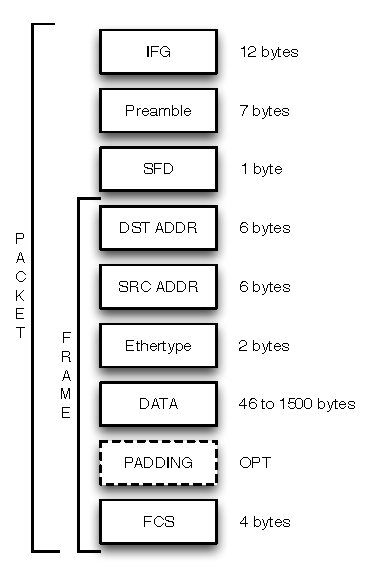
\includegraphics[scale=1.00,center]{Diagrams/MAC-FRAME.pdf}
  \caption{Ethernet Packet Structure with the \ac{MAC} Protocol}\label{fig:Eth-frame}
\end{figure}

\paragraph*{DST ADDR} The destination address is a 6-byte field that specifies the \ac{MAC} adapter(s) for which the packet shall be delivered, through the use of an unicast or multicast address.

\paragraph*{SRC ADDR} The source address is a 6-byte field that specifies the unique \ac{MAC} adapter from which the packet is sent.

\paragraph*{Ethertype} This is a 2-byte field\footnote{Type for ARP is 0x0806, for \ac{IP} is 0x0800} field that identifies the type of protocol being carried on the payload.

\paragraph*{Data} This is the field that carries the inner protocol payload.

\paragraph*{Padding} This is an optional field necessary when the Data field is smaller than the specified size of 46 bytes.

\paragraph*{FCS} This is a 4-byte field that contains the \acf{CRC} of the \ac{MAC} frame. The \ac{CRC} is calculated over all fields of the \ac{MAC} frame, except the \ac{FCS} field. The \ac{CRC} uses the 0x04c11db7 polynomial.

The FaceWorks implementation of the \ac{MII} interface and \ac{MAC} layer consists of two logic blocks, an Ethernet receiver and an Ethernet transmitter, as shown in Figure \ref{fig:FW-diag}.

The receiver block is responsible for removing the preamble, detecting the \ac{SFD}, performing packet filtering based on the destination \ac{MAC} and Ethertype, and checking the \ac{CRC} to validate the data.

The inverse operation is performed by the transmitter block: it adds the preamble to the payload, inserts the \ac{SFD}, the Ethernet header, and calculates the trailing \ac{CRC}.

As imposed by the specification, the \ac{MII} interface clock has a period of 40 ns. However, the internal FaceWorks clock period is often faster. Since two clock domains exist, two asynchronous \acp{FIFO} are necessary to buffer the data in each direction.

\section{Address Resolution Protocol}
\nocite{rfc2119}

The \acf{ARP}\cite{rfc826} is used for resolving network layer addresses into data link layer addresses. Since IPv4 over Ethernet is beng used, the correspondence between an \ac{IP} address and a \ac{MAC} address is established. It can also be used for different types of network layer and data link layer protocols.

When a computer A wants to send a packet to a computer B in the \ac{LAN}, it needs to identify it with the \ac{IP} address and the \ac{MAC} address of computer B, to unequivocally tell the computer that is supposed to get this packet.

Assuming that computer A knows the \ac{IP} address of computer B, it sends an \ac{ARP} Request to all computers in the \ac{LAN}, to inquire which computer possesses that \ac{IP} address. Upon receiving the \ac{ARP} Request, computer B replies with an \ac{ARP} Reply packet, which causes computer A to learn the \ac{MAC} address of computer B, and finally send the packet to computer B. To avoid sending an \ac{ARP} Request every time a packet needs to be sent, computer A holds a simple \ac{ARP} cache, where it stores \ac{IP}/\ac{MAC} address pairs. Figure \ref{fig:Arp-eth} shows how an \ac{ARP} packet is structured. This packet format is used for both the \ac{ARP} Request and for the \ac{ARP} Reply. Each field of an \ac{ARP} packet is explained next.

\begin{figure}[h]
  \centering
      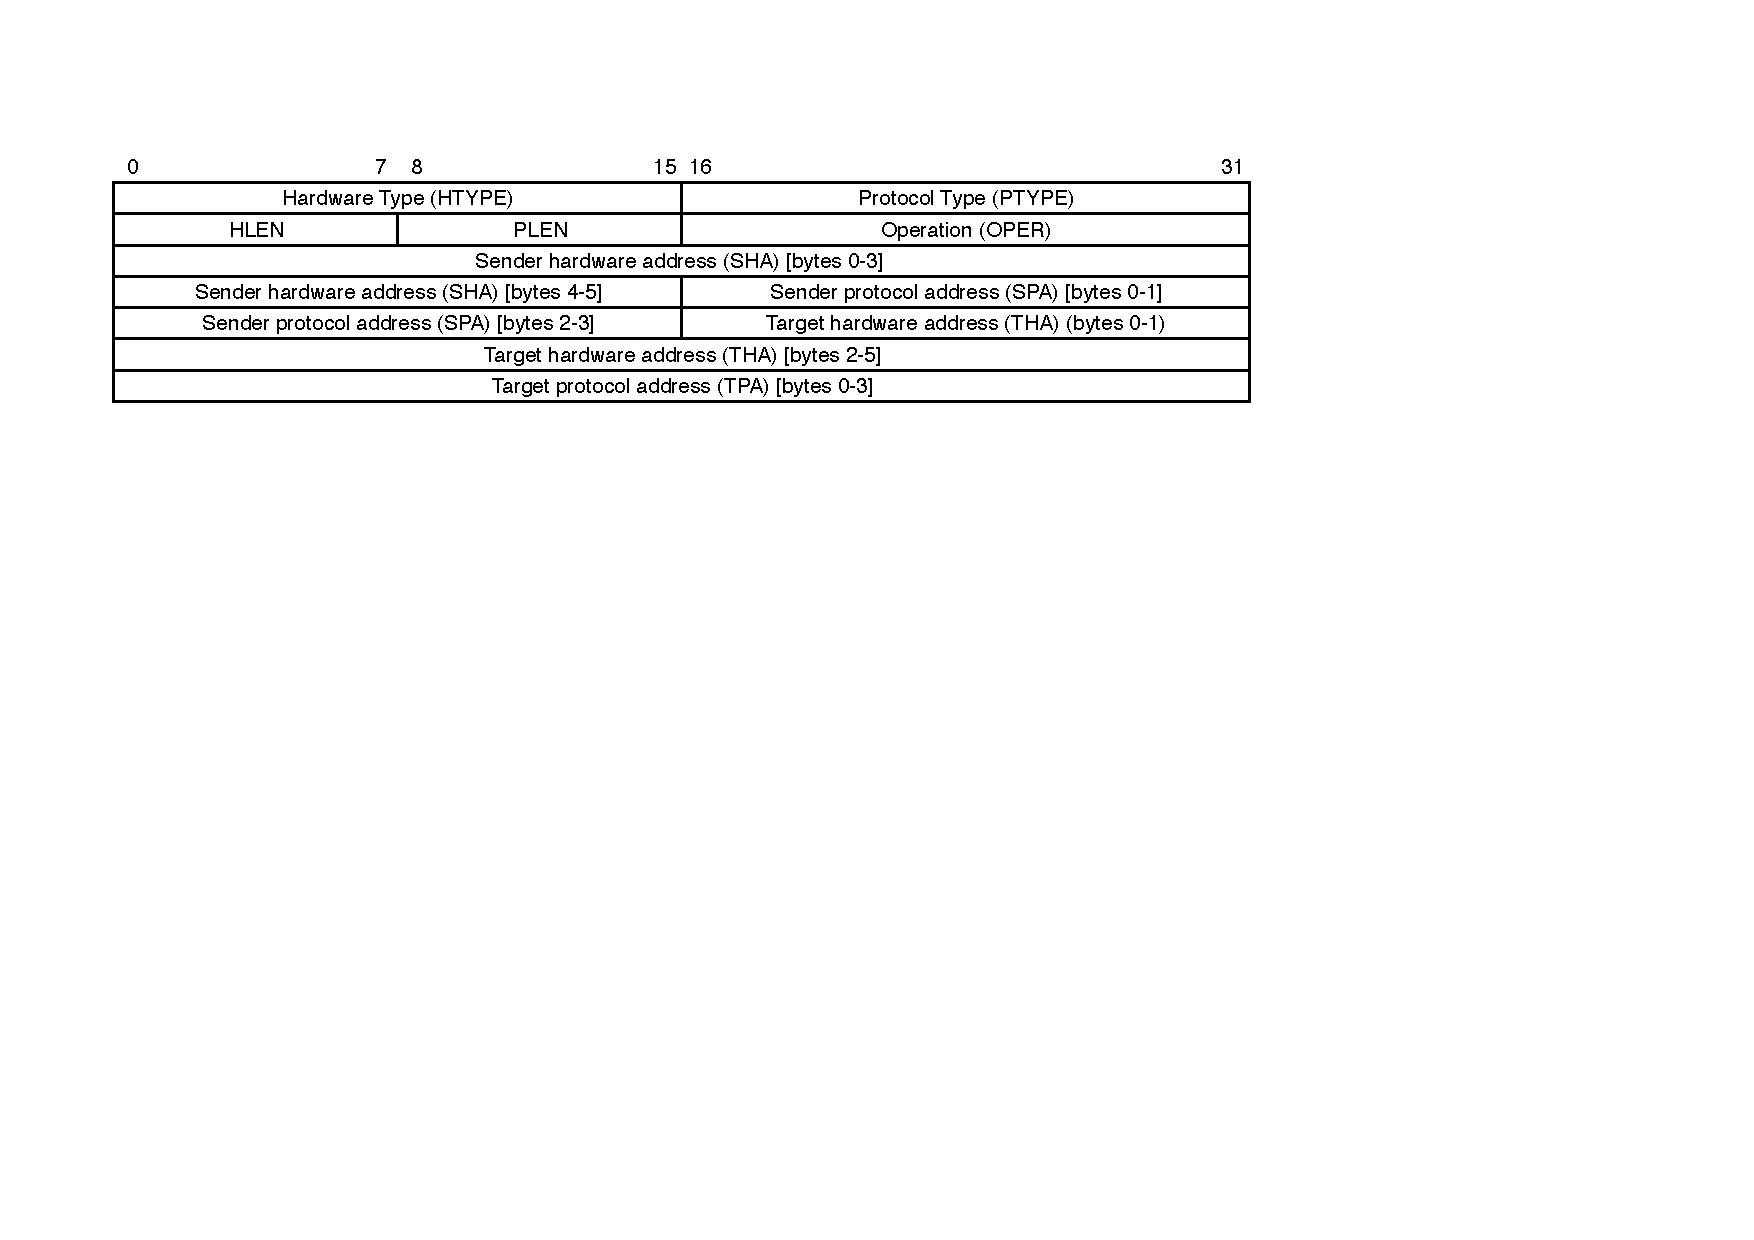
\includegraphics[scale=0.80,center]{Diagrams/ARP.pdf}
  \caption{\ac{ARP} Packet}\label{fig:Arp-eth}
\end{figure}

\paragraph*{HTYPE} The Hardware Type specifies the data link layer protocol type; for Ethernet this value is 0x0001.
\paragraph*{PTYPE} The Protocol Type specifies the network layer protocol; for IPv4 it has the value 0x0800.
\paragraph*{HLEN} The Hardware Length specifies the data link layer address size; for Ethernet this value is 0x06 (length of the \ac{MAC} address).
\paragraph*{PLEN} The Protocol Length specifies the network layer address size; for Ethernet this value is 0x04.
\paragraph*{OPER} The Operation field specifies the type of the \ac{ARP} packet; the value is 1 for an \ac{ARP} Request, 2 for an \ac{ARP} Reply.
\paragraph*{SHA} The Sender Hardware Address contains the sender \ac{MAC} address.
\paragraph*{SPA} The Sender Protocol Address contains the sender \ac{IP} address.
\paragraph*{THA} The Target Hardware Address contains the target \ac{MAC} address; this field is ignored in \ac{ARP} Requests.
\paragraph*{TPA} The Target Protocol Address contains the target \ac{IP} address; this field is ignored in \ac{ARP} Requests.

\vspace{0.5cm}
The FaceWorks \ac{ARP} implementation consists in a single-entry \ac{ARP} table, to create the correspondence between the \ac{IP} address and the \ac{MAC} address of the host that drives FaceWorks. The \ac{ARP} table is connected to both the Ethernet RX and Ethernet TX blocks, as shown in Figure \ref{fig:FW-diag}.

Upon reception of an \ac{ARP} Request, the Ethernet RX block forwards the packet to the ARP block which generates an \ac{ARP} Reply packet and requests the Ethernet TX block to transmit it to the network.

When the Ethernet TX block is constructing an Ethernet packet to be sent, it provides the destination \ac{IP} of the host to the \ac{ARP} logic. If the \ac{IP} is registered in the table, the ARP block outputs the host \ac{MAC} address; otherwise the \ac{ARP} block generates an \ac{ARP} Request, which is sent by the Ethernet TX block. Later, the respective \ac{ARP} Reply will be processed by the Ethernet RX block, which forwards the \ac{IP} and \ac{MAC} address to the \ac{ARP} block. After this the \ac{ARP} table holds the necessary information to process the current and future Ethernet TX requests to the same host.
\clearpage
Figure \ref{fig:Arp-example} exemplifies how values are assigned to the \ac{ARP} packet fields: computer A with \ac{IP} address 192.168.0.22 and \ac{MAC} address 00:26:9e:e2:e3:14 broadcasts an \ac{ARP} Request to find \ac{IP} address 192.168.0.133, and receives a reply from FaceWorks containing its \ac{MAC} address.

\begin{figure}[h]
  \centering
      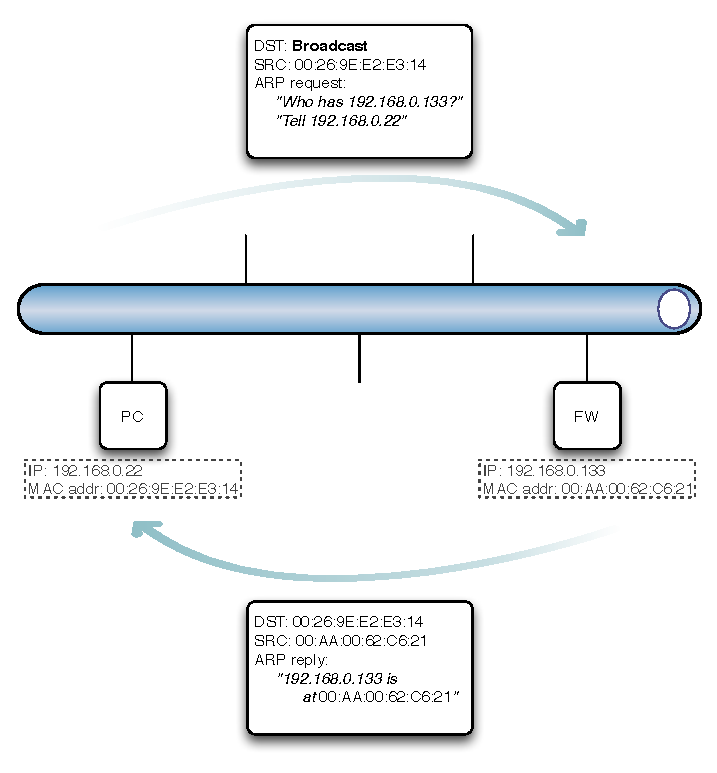
\includegraphics[scale=0.75,center]{Diagrams/ARP-example.pdf}
  \caption{Address Resolution using \ac{ARP}}\label{fig:Arp-example}
\end{figure}
\section{Internet Protocol}

The \acf{IP}\cite{rfc791} main purpose is to provide an abstraction layer that hides differences on the data link layer implementation. It offers a uniform addressing and routing scheme, and a fragmenting mechanism so that different \ac{MTU} values can be supported across different data link layer technologies. FaceWorks only supports IPv4 packets; therefore, IPv6 packets are not discussed here. An IP packet consistes of header and payload. Figure \ref{fig:ipv4} shows the format of an IPv4 packet header. The meaning of each field is explained below.

\begin{figure}[h]
  \centering
      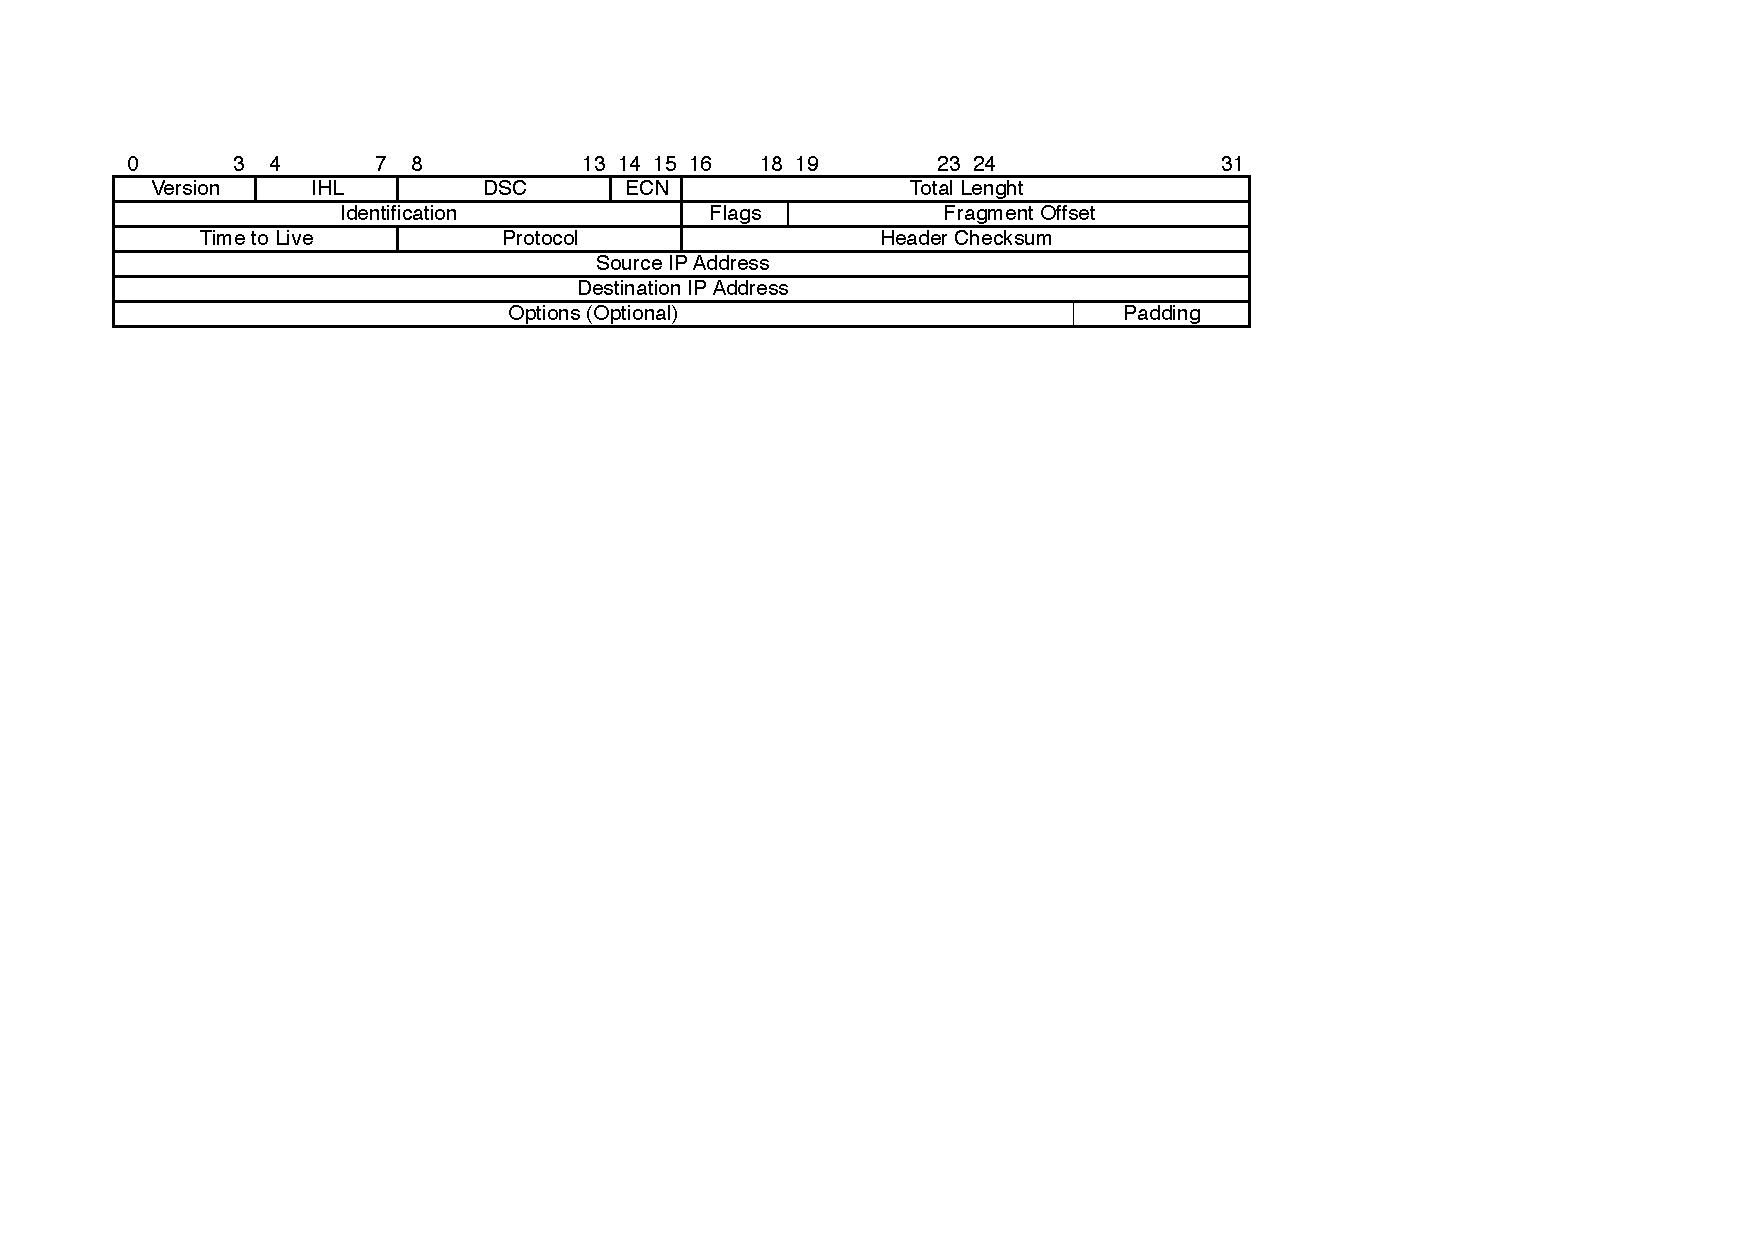
\includegraphics[scale=0.80,center]{Diagrams/IP-Packet.pdf}
  \caption{IPv4 Packet Header}\label{fig:ipv4}
\end{figure}

\paragraph*{Version} This 4-bit field identifies the version number of the Internet Protocol, only versions v4 and v6 are defined. For IPv4 this value is 4.
\paragraph*{IHL} The Internet Header Length is also a 4-bit field that contains the length of the packet header in 32-bit words, and points to the beginning of the data. The smallest valid value is 5 and the highest value is 15 (corresponds to a header length of 60 bytes).
\paragraph*{DSC} The Differentiated Services Codepoint is a 6-bit field used for describing the intended forwarding behavior. This is mainly used for real-time applications, and is not used in FaceWorks.
\paragraph*{ECN} The Explicit Congestion Notification is a 2-bit optional field, which is an extension to \acs{TCP}/\ac{IP} used for end-to-end congestion notification. This field is not supported by FaceWorks.
\paragraph*{Total Lenght} This is the total length of the \ac{IP} packet. It is a 16-bit field, so the maximum size of an \ac{IP} datagram is 65535 bytes. The minimum-length of a packet is 20 bytes (size of header without data). The largest datagram size that a IP-enabled computer is required to reassemble is 576 bytes.
\paragraph*{Fragment ID} The destination computer uses this identifier and the sender's address to identify fragments of \ac{IP} datagrams, so that the original datagrams are reconstructed at the destination computer. FaceWorks does not support \ac{IP} fragmentation.
\paragraph*{Flags} The flag field is used for fragmented \ac{IP} packets. It contains two flags: Don't Fragment (DF) and More Fragments (MF). The DF bit shows that the datagram must not be fragmented, even if it cannot be forwarded further. The MF bit shows more fragments exist in this \ac{IP} packet. Thus, the last packet of a fragmented \ac{IP} datagram has MF set to 0. Both these flags are not supported in the FaceWorks \ac{IP} implementation.
\paragraph*{Fragment Offset} Specifies where in reference to the beginning of the entire datagram the present fragment has to be ordered. This information is essential to reassemble the original packet from the individual fragments in the case fragments arrive out-of-order This is also not supported by the FaceWorks \ac{IP} implementation.
\paragraph*{TTL} The Time To Live is an 8-bit field that is used to prevent datagrams from going in circles in the internet. It implements a counter that for each router on the path is decremented by at least one. If the field reaches value 0, then the packet is discarded.
\paragraph*{Protocol} An 8-bit field that describes the protocol used in the payload of the \ac{IP} datagram.\footnote{UDP is 17} 
\paragraph*{Header Checksum} This field contains a 16-bit checksum of the \ac{IP} packet header. It is used for error-checking the \ac{IP} header. When a router receives an \ac{IP} packet it calculates the checksum and compares it with the value in this field. If the values match the TTL is decremented by 1 and the checksum has to be updated since the header content has been updated. Since the payload data is not verified by this checksum, the payload protocols have their own checksum.
\paragraph*{Sender Address} This field contains the 32-bit \ac{IP} address of the sender computer.
\paragraph*{Destination Address} This field contains the 32-bit \ac{IP} address of the destination computer.
\paragraph*{Options} This field is used for user data, and must comply with a standard format not discussed here. Since the header length must be a 32-multiple, the user is required to insert padding bits. This field not used or supported by FaceWorks.

%Nunca mas nunca usar elisões em linguagem formal: isn't NAO is not SIM 
\vspace{10pt}
The implementation of the \ac{IP} protocol in FaceWorks uses two blocks, the \ac{IP} RX block and the \ac{IP} TX block, as depicted in Figure \ref{fig:FW-diag}. 

The \ac{IP} RX block implements the \ac{IP} protocol for the receive packets. It processes the \ac{IP} packets that are received from the \ac{MAC} layer, according to the values of their \ac{IP} header version, destination \ac{IP} address and protocol type. It calculates the checksum to verify the header and forwards the payload data to the next block, the \ac{UDP} RX block.

For transmit packets the \ac{IP} TX block calculates the header checksum and writes the \ac{IP} header and checksum in the \acs{RAM} TX block, which is where the packet is being formed. Finally, it requests the Ethernet TX module to send the packet.


\section{User Datagram Protocol}

The \acf{UDP}\cite{rfc768} provides an unreliable, connectionless transport datagram service. \ac{UDP} uses the Internet Protocol as the underlying protocol.

\ac{UDP} is suitable for this work because error checking is not necessary, and retransmission of lost packets is implemented by a higher application protocol. This way the overhead of a TCP session is avoided, and a much simpler implementation on the hardware is obtained. 



\subsection{\ac{UDP} Packet Header}

A UDP packet consists of header and payload. Figure \ref{fig:udp} shows the format of a \ac{UDP} packet header. The header fields are briefly described below.

\begin{figure}[h]
  \centering
      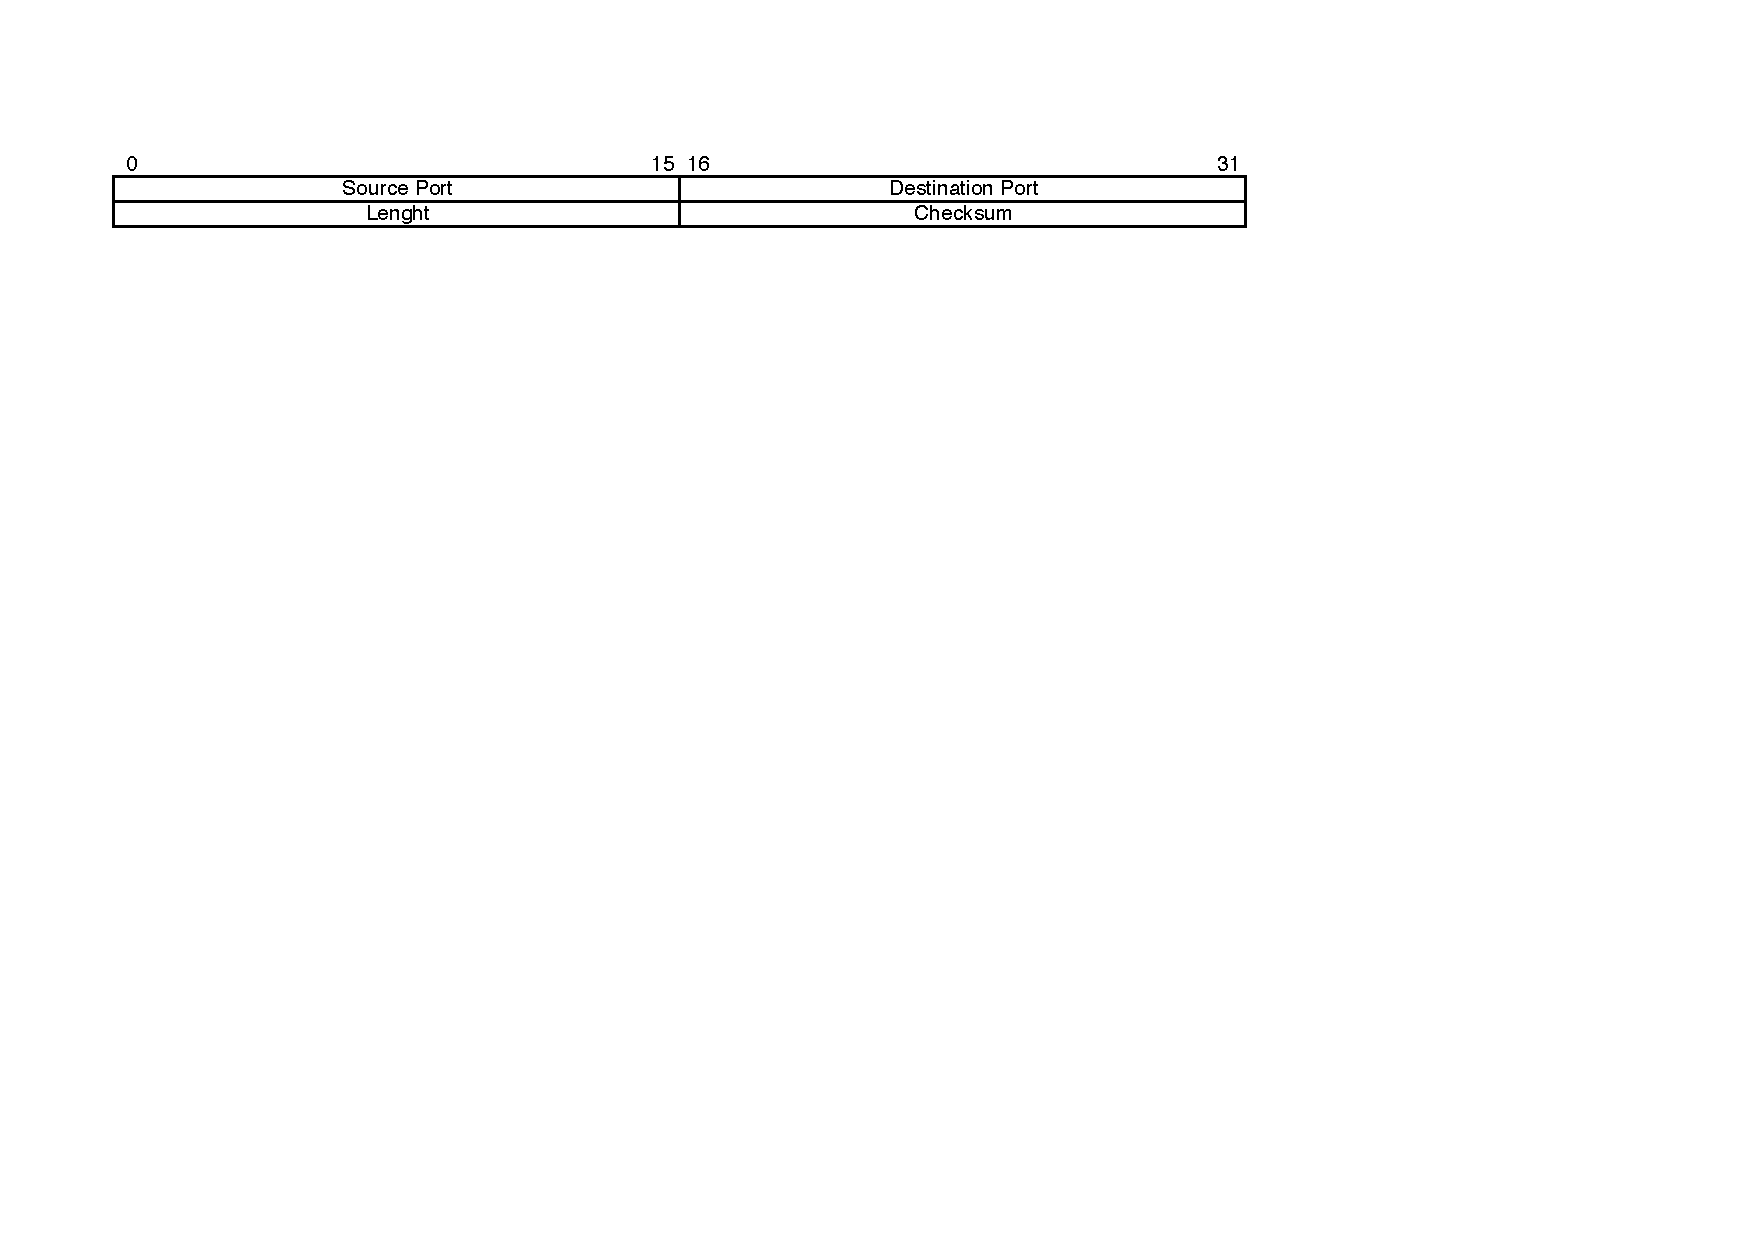
\includegraphics[scale=0.8,center]{Diagrams/UDP-Header.pdf}
  \caption{\ac{UDP} Packet Header}\label{fig:udp}
\end{figure}

\paragraph*{Source Port} This is a 16-bit field which identifies the port used by the sender process.
\paragraph*{Destination Port} This is a 16-bit field that identifies the destination port used by the receiver process.
\paragraph*{Length} This is a 16-bit field, which contains the size in bytes of the packet header and payload combined.
\paragraph*{Checksum} This a field used for verifying the contents of the header and data. The checksum is calculated over a pseudo-header, the \ac{UDP} header and the data. Padding may be necessary in order to have multiples of two bytes.

\subsection{Implementation}

The FaceWorks implementation for the transport layer is also composed of two blocks,  the \ac{UDP} RX and the \ac{UDP} TX blocks, as shown in Figure \ref{fig:FW-diag}.

The \ac{UDP} RX block filters out \ac{UDP} messages that are not being sent to the \ac{UDP} port being used for \ac{CWDP} communication. For messages addressed to the \ac{UDP} port being used for \ac{CWDP} communication, the \ac{UDP} RX block removes the \ac{UDP} header and forwards the \ac{UDP} payload (\ac{CWDP} packet) to the \ac{CWDP} RX module. 

The \ac{UDP} TX block inserts the \ac{UDP} header in the \acs{RAM} TX buffer, calculates the checksum assuming the pseudo-header is attached upfront, and forwards the transmission of the \ac{UDP} packet to the \ac{IP} TX module.
\clearpage
\section{Coreworks Datagram Protocol}

The \acf{CWDP}\cite{Facedata} is a proprietary protocol, which runs over \ac{UDP}, and was created to communicate with the on-chip cores using the FaceWorks core. Each \ac{CWDP} packet is sent as a \ac{UDP} payload, as shown in Figure \ref{fig:cwdp-encap}.

\begin{figure}[h]
  \centering
      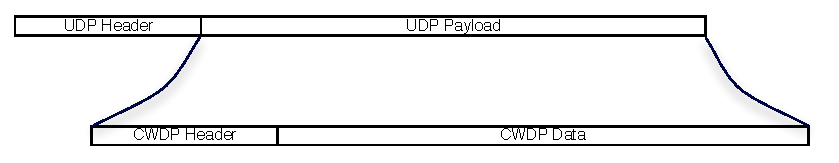
\includegraphics[scale=1]{Diagrams/CWDP-Encap.pdf}
  \caption{\ac{CWDP} Encapsulation in the \ac{UDP} Payload}\label{fig:cwdp-encap}
\end{figure}

For this project only a subset of the FaceWorks commands is presented, since there are several features that have not been used in this work.

\subsection{CWDP Packet}

Figure \ref{fig:cwdp-packet} shows how a \ac{CWDP} packet is structured. The fields are briefly described below

\begin{figure}[h]
  \centering
      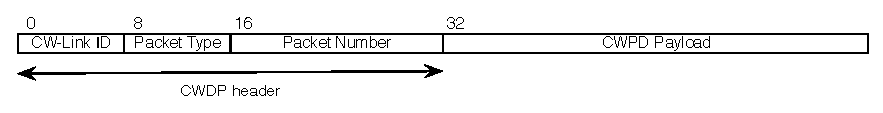
\includegraphics[scale=1]{Diagrams/CWDP-Packet.pdf}
  \caption{\ac{CWDP} Packet}\label{fig:cwdp-packet}
\end{figure}

\paragraph*{CW-Link ID} This field identifies the destination core interface for which the packet data is intended.
\paragraph*{Packet Type} This field identifies the CWDP packet type; not all available packet types are used in this work.
\paragraph*{Packet Number} This field is a sequence number for data packets. It is used to implement reliable transmission. The Packet Number is incremented for every packet acknowledged by the receiver. Only packets with the expected Packet Number are acknowledged by the receiver.
\paragraph*{Payload} Contains the data to be delivered to the cores, or parameters for FaceWorks.

\subsection{Packet Types}

This section presents the \ac{CWDP} packet types that have been used in this work. Refer to \cite{Facedata} for a complete outline of the existing CWDP packet types.

% %START CORE ACCESS
\paragraph*{SET\_CORE\_ACCESS} (packet type 0x03) This packet type is used to initialize the FaceWorks core. In Figure \ref{fig:cwdp-core-access} the structure of a \ac{CWDP} SET\_CORE\_ACCESS packet is shown. When a \ac{CWDP} SET\_CORE\_ACCESS packet is received by FaceWorks it locks to the host \ac{IP} and \ac{UDP} port of the origin for the purpose of replying. The \ac{ARP} table is cleared and any packet present in the receive or transmit buffers are deleted. Incoming or outgoing packet counters are both reset to zero. The registered host will maintain control of FaceWorks core until a \ac{CWDP} SET\_MAC packet is sent by the host. When FaceWorks is locked to a host, other incoming \ac{CWDP} packets from other origins are dropped.


\begin{figure}[h]
  \centering
      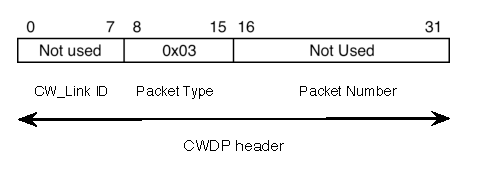
\includegraphics[scale=1]{Diagrams/CWDP-Set-core-access.pdf}
  \caption{\ac{CWDP} SET\_CORE\_ACCESS Packet}
  \label{fig:cwdp-core-access}
\end{figure}


\paragraph*{SET\_MAC} (packet type 0x04) This type is now used to release control and terminate a connection with the FaceWorks core. In a complete FaceWorks implementation this could be used to change from core access mode to \ac{MAC} mode. In \ac{MAC} mode FaceWorks as a regular MAC core by an embedded processor and CORE\_DATA packets can not be transmitted.  In Figure \ref{fig:mac-access} the structure of the \ac{CWDP} SET\_MAC packet is shown. When a \ac{CWDP} SET\_MAC packet is received the control of the FaceWorks core is released, the registered \ac{IP} and \ac{UDP} port are deleted, the \ac{ARP} table is cleared and packet buffers are cleared. Incoming or outgoing packet counters are both reset to zero. Control can be regained by sending a SET\_CORE\_ACCESS packet again.

\begin{figure}[h]
  \centering
      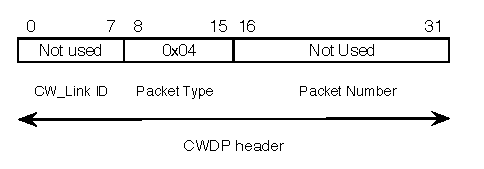
\includegraphics[scale=1]{Diagrams/CWDP-Set-MAC.pdf}
  \caption{\ac{CWDP} SET\_MAC Packet}
  \label{fig:mac-access}
\end{figure}

\paragraph*{CORE\_DATA} (packet type 0x01) This packet type is used to send data between systems and cores. In Figure \ref{fig:cwdp-data} a \ac{CWDP} CORE\_DATA packet is shown. The packet payload is composed of several CW-Link words, each word is 32-bit long and each CORE\_DATA packet can contain up to 360 CW-Link words.
% %ACK

\begin{figure}[h]
  \centering
      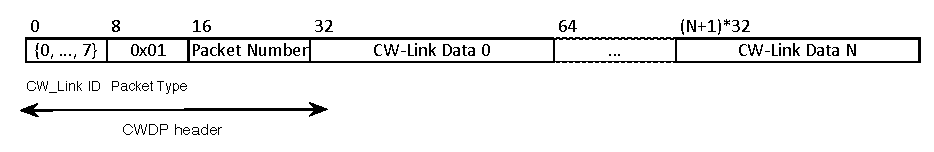
\includegraphics[scale=1,center]{Diagrams/CWDP_Core_data_paper.pdf}
  \caption{\ac{CWDP} CORE DATA Packet}
  \label{fig:cwdp-data}
\end{figure}


\paragraph*{ACK} (packet type 0x02) This packet type is used to acknowledge received packets. In Figure \ref{fig:cwdp-ack}, the structure of a \ac{CWDP} ACK packet is shown. Received \ac{CWDP} packets, except for the \ac{ACK} packet itself, trigger a reply with an \ac{ACK} packet. The packet number of the transmitted \ac{ACK} matches the packet number of the received packet when a CORE DATA packet is received. If the received packet is a SET\_CORE\_ACCESS packet then the packet number of the \ac{ACK} packet is set to zero.

\begin{figure}[h]
  \centering
      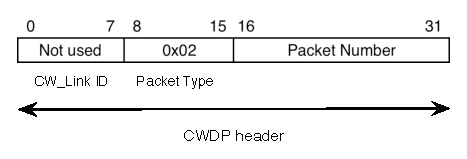
\includegraphics[scale=1]{Diagrams/CWDP-Ack.pdf}
  \caption{\ac{CWDP} ACK Packet}
  \label{fig:cwdp-ack}
\end{figure}
\clearpage


\subsection{Implementation}

The \ac{CWDP} application layer is implemented using 4 logic blocks (\ac{CWDP} RX, \ac{CWDP} TX, CW-Link RX and CW-Link TX), as shown in Figure \ref{fig:FW-diag}.

The \ac{CWDP} RX block implements the \ac{CWDP} protocol for the received packets. It decodes the type of the received packet and performs the instructed action. The payload of CORE\_DATA packets is placed in the \acs{RAM} RX buffer. After the reception of a \ac{CWDP} packet it requests the \ac{CWDP} TX to send the acknowledge packet. If the \ac{CWDP} packet is a CORE DATA packet it forwards the data to CW-Link RX block in order to be delivered to the addressed \ac{IP} Core. An interaction diagram between the CWDP receive and transmit sides is shown in Figure \ref{fig:cwdp-transac}.

\begin{figure}[h]
  \centering
      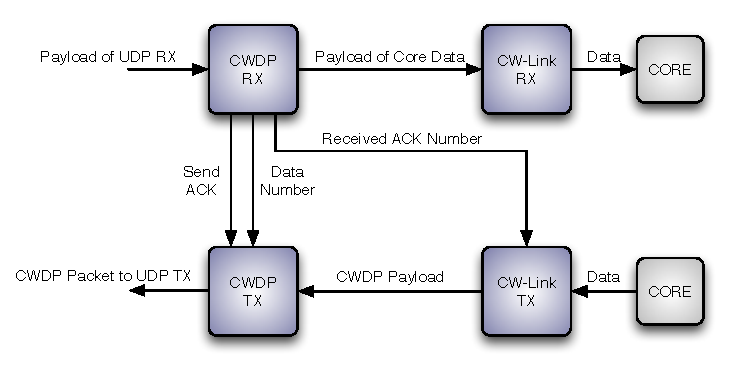
\includegraphics[scale=1]{Diagrams/CWDP-simplified-transaction.pdf}
  \caption{\ac{CWDP} Layer}
  \label{fig:cwdp-transac}
\end{figure}

The \ac{CWDP} TX block receives data from the CW-Link TX block and sends the data to the \ac{UDP} TX module by means of the \acs{RAM} TX buffer. Then it waits for the \ac{ACK} packet of the sent packet, which will arrive in the \ac{CWDP} RX block. When the \ac{ACK} packet arrives, the \ac{CWDP} RX block presents the sequence number to the \ac{CWDP} TX block, so it can verify that it matches the sequence number of the packet previously sent.
\clearpage

\subsection{CW-Link Interface}
FaceWorks uses CW-Link interfaces\cite{Facedata} to send data or commands to and from the cores inside the chip. In Figure \ref{fig:cwdp-diagram} the CW-Link interfaces between FaceWorks and a few cores are shown.

\begin{figure}[h]
  \centering
      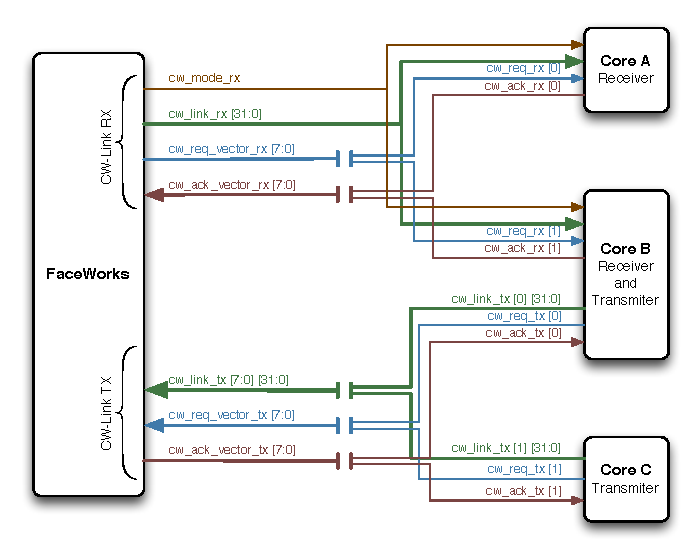
\includegraphics[scale=1.3]{Diagrams/CW-Link-Diag.pdf}
  \caption{CW-Link Interface}
  \label{fig:cwdp-diagram}
\end{figure}


The CW-Link interfaces specifies four logic signals: request ({\tt req}), acknowledge (\texttt{ack}), data (\texttt{link}) and mode (\texttt{mode}). FaceWorks is the master of the CW-Link RX interface and is a slave of the CW-Link TX interface. The mode signal is only used in the CW-Link RX interface to distinguish between data and commands for the \ac{ILP} cores. The CW-Link RX may be interconnected to eight different \ac{ILP} cores. 

As depicted in Figure \ref{fig:cwdp-diagram} both the receive data bus and mode signal are shared between the receiving cores, and there is a \texttt{req}/\texttt{ack} pair for each of the 8 cores; only one of the  \texttt{req} signals may be active at any instant. There is one transmit data bus and one \texttt{req}/\texttt{ack} pair for each core.

A timing diagram of CW-Link RX transactions is shown in Figure \ref{fig:tim-cw}. The communication uses simple handshaking: a single bit from the \texttt{req} signal vector goes high to identify the destination \ac{ILP} core while the data bus holds a valid value until the respective \texttt{ack} signal goes high.

\begin{figure}[h]
  \centering
      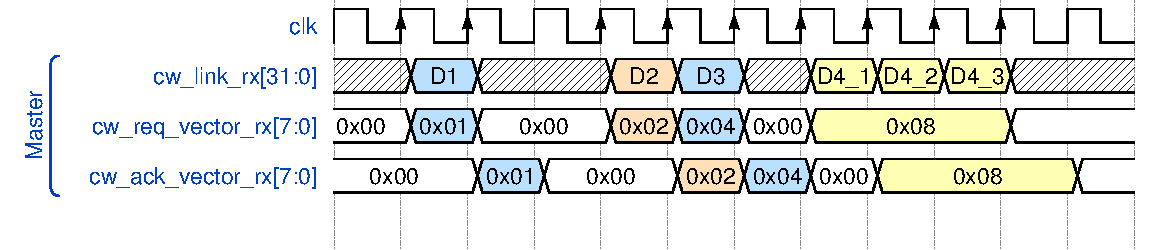
\includegraphics[scale=0.8,center]{images/fw-time.pdf}
  \caption{CW-Link RX Transactions}\label{fig:tim-cw}
\end{figure}

CW-Link also supports burst transfers by keeping the request signal high and sending data words
consecutively as long as the \texttt{ack} signal is kept high. An example burst transfer is depicted in yellow in Figure \ref{fig:tim-cw}\footnote{This timing diagram has been constructed using the javascript web application Wavedrom available at: http://wavedrom.googlecode.com} and consists of 3 data words for core 4.
The same rationale is used for the CW-Link TX interface.



% Ensure that the next chapter starts in a odd page
\cleardoublepage

% %%%%%%%%%%%%%%%%%%%%%%%%%%%%%%%%%%%%%%%%%%%%%%%%%%%%%%%%%%%%%%%%%%%%%%
% Your work: Chapter 3
% %%%%%%%%%%%%%%%%%%%%%%%%%%%%%%%%%%%%%%%%%%%%%%%%%%%%%%%%%%%%%%%%%%%%%%
\fancychapter{Design}

In this chapter the implementation of multiple \ac{UDP} ports for FaceWorks is presented. The software components and the hardware modifications effected to support two distinct ports are explained. The same method can be used for more than two ports.

During the development loopback wires have been used, to directly connect the CW-Link RX block to the CW-Link TX block, as shown in Figure \ref{fig:CW-LoopBack}. With the CW-Link loopback, there is no need for a stimulus generator for the CW-Link TX interface. CORE\_DATA packets are sent from a host computer and are delivered back to the host. This way packets that are sent and received back can be compared to detect possible differences.

\begin{figure}[h]
  \centering
      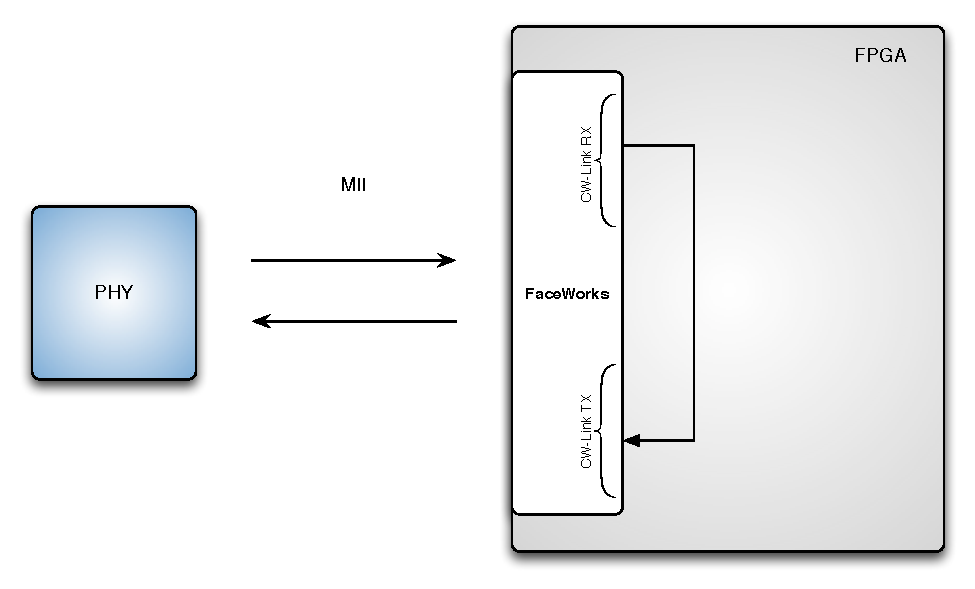
\includegraphics[scale=0.70]{Diagrams/CW-LoopBack.pdf}
  \caption{CW-Link Loopback}\label{fig:CW-LoopBack}
\end{figure}



\section{Face-Test Application}

The FaceWorks test application (Face-Test) is a C language application that implements the \ac{CWDP} protocol. The application has been tested on the pre-existing FaceWorks architecture and on the new FaceWorks architecture.

\subsection{Basic Functions}
The two basic functions used in the Face-Test application are the {\tt CWDP\_receive\_packet()} and the {\tt CWDP\_send\_packet()} functions. These functions create an abstraction layer which hides the \ac{CWDP} details. They are used for sending / receiving packets to / from FaceWorks, and can be called for different sessions/connections inside a user process.


The \texttt{CWDP\_receive\_packet} function (Figure \ref{fig:drivers}) reads \ac{UDP} packets from a socket descriptor {\tt fd} and places the content in buffer {\tt buf\_in}. If the received packet is an \ac{ACK} packet the value of {\tt core\_out} (sequence number of the last packet sent) is compared with the sequence number of the received ACK packet. If they do not match the {\tt CWDP\_receive\_packet()} function returns the error code {\tt P\_ERROR}; otherwise the function returns the type of packet received. If a {\tt CORE\_DATA} packet is received the {\tt ack\_out} variable is updated with the sequence number of the received {\tt CORE\_DATA} packet so a \ac{ACK} packet can be sent with the correct value.

\begin{figure}[h]
\begin{boxedverbatim}
int CWDP_receive_packet (int fd, struct sockaddr_in server_addr,byte *buf_in,
u_int16_t *core_out,u_int16_t *ack_out);
int CWDP_send_packet (int fd, struct sockaddr_in addr, struct sockaddr_in server_addr, byte *buf_out,
byte * buf_in, int buf_size, e_cwdp cwdp_type, u_int16_t *core_out, u_int16_t *ack_out);
\end{boxedverbatim}
\caption{\ac{CWDP} Send/Receive Functions}
\label{fig:drivers}
\end{figure}

%corrigir tipos de letras
The CWDP\_send\_packet function (\ref{fig:drivers}) sends a \ac{UDP} packet to a socket descriptor {\tt fd}, using as destination the FaceWorks IP address {\tt addr}.

If the type of packet sent requires an acknowledge from FaceWorks, the {\tt CWDP\_send\_packet()} function internally calls to the {\tt CWDP\_receive\_packet()} function to get the packet, and then verifies if the sequence number is the expected one. 



\subsection{Test Application}

The Face-Test application is a simple C application that consists in sending CORE\_DATA packets with random data from a PC to a network connected \ac{FPGA} with a FaceWorks core.

After defining the socket settings the application starts by sending a SET\_CORE\_ACCESS packet as depicted in Figure \ref{chp3:code_coreaccess} to establish the PC controlling the FaceWorks core.

\begin{figure}[h]
\begin{boxedverbatim}
/*Send Core Access and receive Ack*/
buf_size=0;
CWDP_send_packet (fd,addr,server_addr,buf_out,buf_in,buf_size,P_SET_CORE_ACCESS,&core_out,&ack_out);
\end{boxedverbatim}
\caption{Send Core Access and Wait for Acknowledge}
\label{chp3:code_coreaccess}
\end{figure}


As Ethernet is a best-effort service, a packet sent by the PC can fail to be delivered to FaceWorks, and the acknowledge sent by FaceWorks can fail to be delivered to the PC.

To resolve both these situations it is needed that the \texttt{CWDP\_receive\_packet()} function have a timeout when reading data from the socket. When the CORE\_ACCESS packet sent from the PC is lost in the network, FaceWorks will not reply with the ACK packet.
\clearpage
\begin{figure}[h]
\centering
\subfigure[Recovery from a lost CORE\_ACCESS]{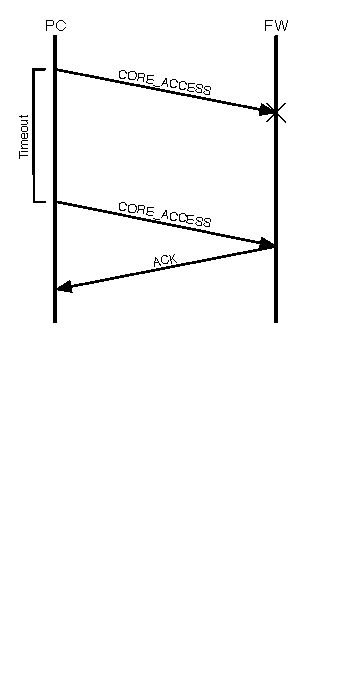
\includegraphics[scale=0.9]{Diagrams/Diag-TO-FW.pdf}\label{fig:Diag-TO-FW}}
\hspace*{2cm}
\subfigure[Recovery from a lost ACK]{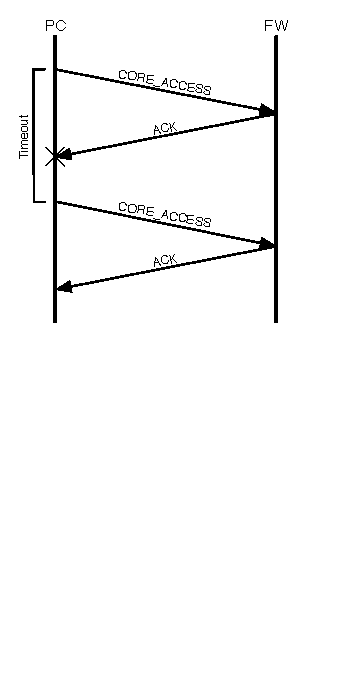
\includegraphics[scale=0.9]{Diagrams/Diag-TO-PC.pdf}\label{fig:Diag-TO-PC}}\\
\caption{Recovering from Lost Packets}
\label{fig:DIAG}
\end{figure}

When the PC is waiting to receive an \ac{ACK} packet from FaceWorks, if a timeout did not exist, the PC would block. Therefore, after a timeout, the \texttt{CWDP\_receive\_packet()} function returns P\_ERROR and the CORE\_ACCESS packet is retransmitted. This situation is depicted in Figure \ref{fig:Diag-TO-FW}.

The same procedure applies for the loss of the \ac{ACK} packet, as depicted in Figure \ref{fig:Diag-TO-PC}. Assuming the \ac{ACK} packet transmitted by FaceWorks is lost in the network, the PC waits for it until the \texttt{CWDP\_receive\_packet()} function times out and returns P\_ERROR. After that, the CORE\_ACCESS packet is retransmitted.

After the PC sends the SET\_CORE\_ACCESS packet to FaceWorks successfully, it can start to send CORE\_DATA packets. To accomplish this the \texttt{CWDP\_send\_packet()} function is called as shown in Figure \ref{chp3:code_coredata}.

\begin{figure}[h]
\begin{boxedverbatim}
/*Send Core Data and receive Ack*/
CWDP_send_packet(fd,addr,server_addr,buf_out,buf_in,buf_size,P_CORE_DATA,&core_out,&ack_out);
\end{boxedverbatim}
\caption{Send Core Data and Wait for Acknowledge}
\label{chp3:code_coredata}
\end{figure}

\clearpage
Now the PC expects to receive the same CORE\_data packet it sent to FaceWorks. To accomplish this the \texttt{CWDP\_receive\_packet()} function is called inside a {\tt do while} loop until a CORE\_DATA packet type is received (Figure \ref{chp3:code_readca_sndack}).
\vspace{3cm}
\begin{figure}[h]
\begin{boxedverbatim}
/*Read Core Data and send Ack*/
do{
    do{
        memset((void*)&buf_in,(unsigned char)0,sizeof(buf_in));
      }while(CWDP_receive_packet(fd,server_addr,buf_in,&core_out,&ack_out)!=P_CORE_DATA);

      CWDP_send_packet(fd,addr,server_addr,buf_out,buf_in,buf_size,P_ACK,&core_out,&ack_out);

      /*Compare sent packet with received packet*/
      if(memcmp(&buf_out[4],&buf_in[4],1444)==0)
      {
#ifdef PREF_TEST
            printf("Data Match!!\n");
#endif
            (u_int16_t)(core_out)++;
      }
      else
      {     
            printf("Invalid Data!!\n");
      }
#ifdef PREF_TEST
      printf("Core seq number: %d Ack seq number: %d\n",core_out,ack_out);
#endif
}while(memcmp(&buf_out[4],&buf_in[4],1444)!=0);
\end{boxedverbatim}
\caption{Read Core Access and Send Acknowledge}
\label{chp3:code_readca_sndack}
\end{figure}

\clearpage

When the CORE\_DATA packet is received from FaceWorks, the PC replies with an \ac{ACK} packet. If this \ac{ACK} packet is not delivered, the PC will not know of this and will transmit the next CORE\_DATA packet.

\begin{figure}[h]
  \centering
      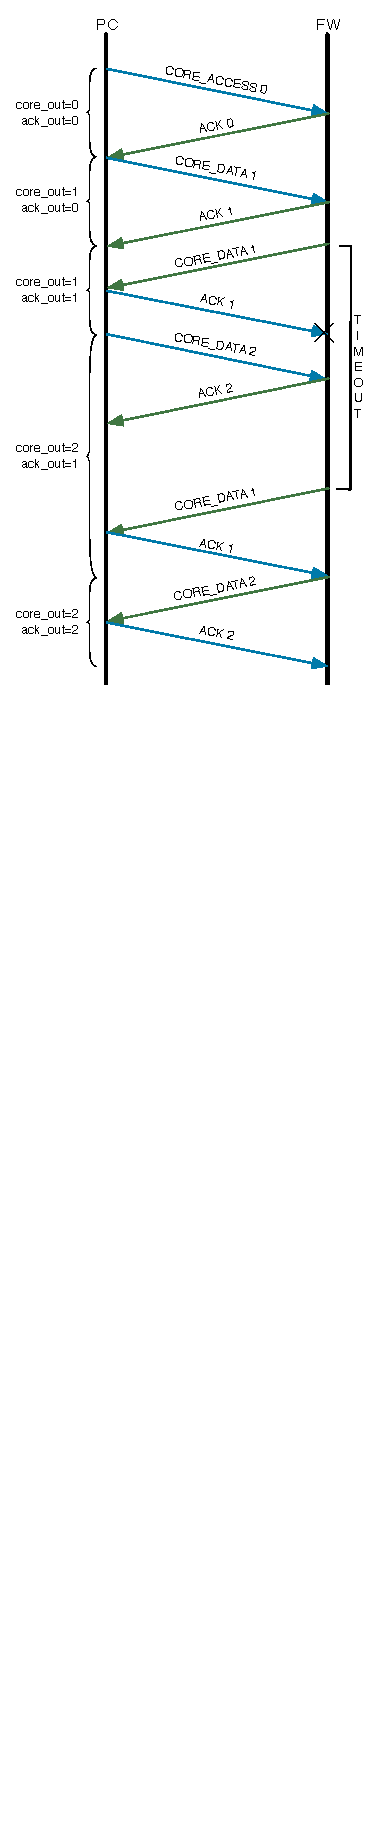
\includegraphics[scale=1.2,center]{Diagrams/Diag-EX.pdf}
  \caption{Facework Recovery from a Lost Packet}\label{fig:Diag-EX}
\end{figure}


FaceWorks assumes the previous CORE\_DATA packet sent was not received by the host, so after a timeout period it resends the same CORE\_DATA packet. A recovery from such failure is depicted in the network diagram in Figure \ref{fig:Diag-EX}.

% Ensure that the next chapter starts in a odd page
\clearpage

\section{Hardware Implementation}

The new architecture is presented in Figure \ref{fig:FW-Final}. Compared to the original architecture, the CWDP\_Link modules are duplicated on both the reception and transmission sides.  The RAM\_RX block is also duplicated in order to receive and store two consecutive packets with different destination ports. An arbiter is added to decide which of the CW-Link TX is granted access to the medium.

%o arbitro nao controla o tx na figura ....
% já foi esclarecido

\begin{figure}[h]
  \centering
      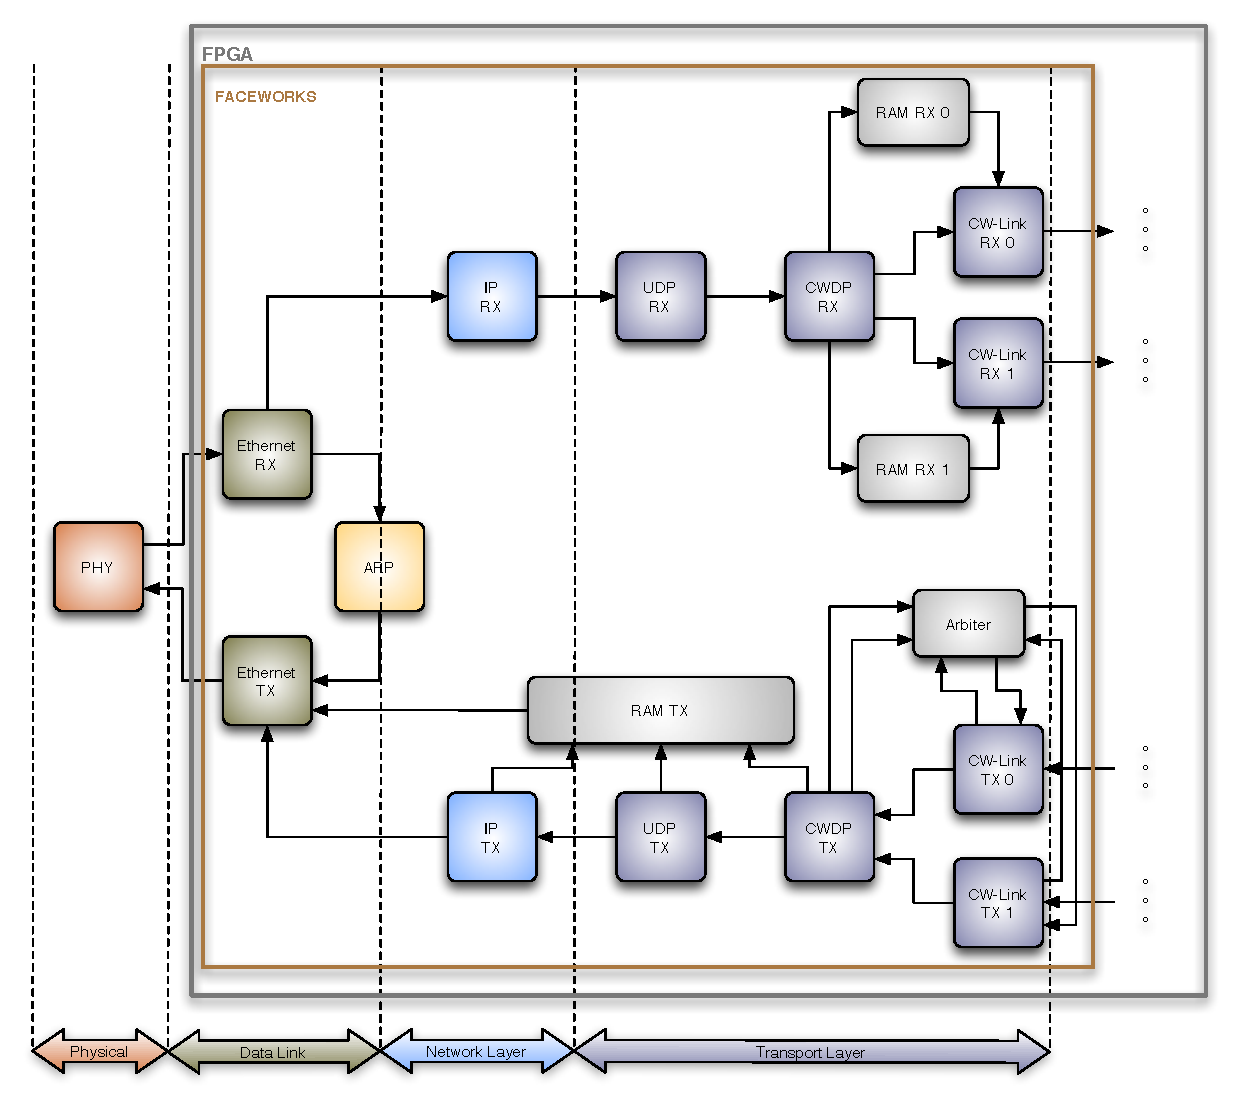
\includegraphics[scale=0.8,center]{Diagrams/FW-Final.pdf}
  \caption{Two-Port FaceWorks Block Diagram}\label{fig:FW-Final}
\end{figure}
\clearpage
\subsection{Modified Blocks}

In this implementation FaceWorks supports a single sender \ac{IP} address and listens to two hardwired \ac{UDP} ports, whose numbers differ by 1. For example, ports 1234 and 1235. The following paragraphs describe the modifications effected on the original hardware blocks.

\paragraph*{\ac{UDP} RX} The \ac{UDP} RX block original implementation filtered out the \ac{UDP} packets whose destination port did not match the current listening port. This behavior has been modified. The \ac{UDP} destination port field is subtracted from the base listening port. If the result is 0 then the packet is aimed at the first port; else, if the result is 1 the packet is aimed at the second port; otherwise the packet is dropped.

\paragraph*{CWDP RX} The \ac{CWDP} RX block is used for both ports and it must keep track of the packet sequence numbers for the two ports. A block diagram is depicted in Figure \ref{fig:CWDPRXDETAIL}. The control signal {\tt CWLinkPort} produced by the \ac{UDP} RX block identifies the currently active port, and is used to select the packet sequence number register to check and increment. The \texttt{CWLinkPort} signal is also decoded to produce a 2-bit signal (\texttt{active\_unit\_RX}) to select the active CW-Link RX block. Upon reception of a SET\_CORE\_ACCESS packet from a given \ac{UDP} port, one of two registers named {\tt( locked\_UDP\_0} and {\tt locked\_UDP\_1)} is set with the source \ac{UDP} port. These are provided to the \ac{CWDP} TX block so it can choose the correct destination \ac{UDP} port to reply to. See Figure \ref{fig:CWDPSIMP2} for details.

% esta figura é deficiente na espessura das linhas
%done
%@HERE

\begin{figure}[h]
  \centering
      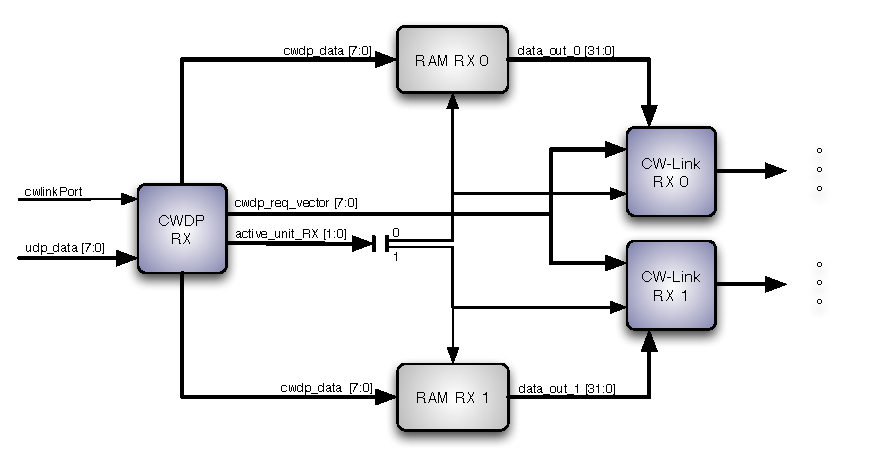
\includegraphics[scale=1.2,center]{Diagrams/CWDP-RX-Detail.pdf}
  \caption{\ac{CWDP} RX and CW-Link RX}\label{fig:CWDPRXDETAIL}
\end{figure}


\paragraph*{CW-Link RX} The CW-Link RX unit is duplicated, one for each communication port. Its control \ac{FSM} has been modified so that they are activated one at a time, based on the value of the control signal {\tt active\_unit\_RX}.

\paragraph*{CW-Link TX} The CW-Link TX unit is duplicated. Its control \ac{FSM} has been modified to allow execution only when the Arbiter block grants access to the (\acs{RAM} TX and \ac{CWDP} TX) resources. To do this, two signals are sent to the arbiter, \texttt{cw\_req\_vector\_TX} and \texttt{busy\_cwlink}, and one signal is received from the arbiter, \texttt{active\_unit\_tx}, as shown in Figure \ref{fig:CWDP-TX}. When the resources are granted to one of the CW-Link TX units the arbiter waits until its execution ends before granting the resources to the other CW-Link TX unit.

\begin{figure}[h]
  \centering
      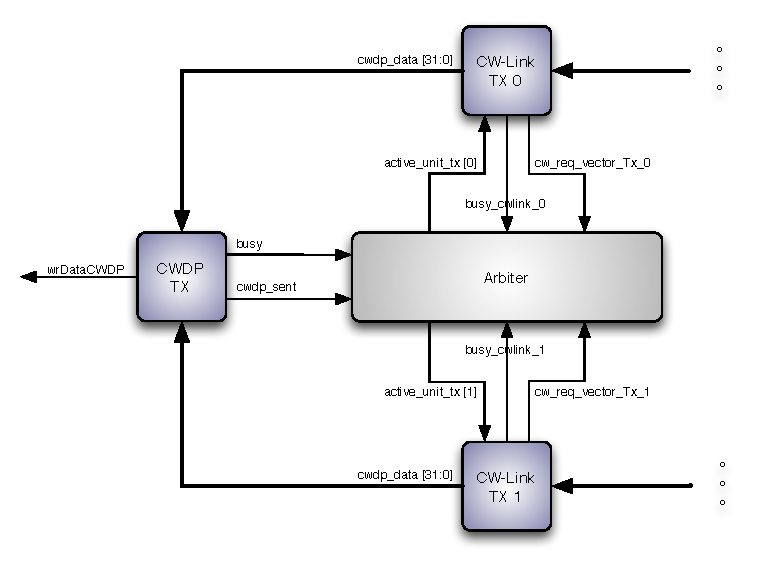
\includegraphics[scale=1.2,center]{Diagrams/CWDP-TX-Detail.pdf}
  \caption{\ac{CWDP} TX and CW-Link TX}\label{fig:CWDP-TX}
\end{figure}

\paragraph*{CWDP TX} A single \ac{CWDP} TX block is used. The \ac{UDP} destination port may be different depending on the type of packet: \ac{ACK} packet requested by the \ac{CWDP} RX block or data packet requested by one of the two CW-Link TX units, as shown in Figure \ref{fig:CWDPSIMP2}. If the \ac{CWDP} TX is processing a CORE\_DATA packet, the destination \ac{UDP} port is selected from the \texttt{locked\_UDP\_0} or \texttt{locked\_UDP\_1} inputs, based on the currently active CW-Link TX block. For an \ac{ACK} packet request, the {\tt SendACK} signal is activated, the {\tt SelACK} signal selects the \ac{UDP} destination port from the \texttt{locked\_UDP\_0} or \texttt{locked\_UDP\_1} inputs, and the sequence number is provided by the {\tt SeqNumACK} signal.

\begin{figure}[h]
  \centering
      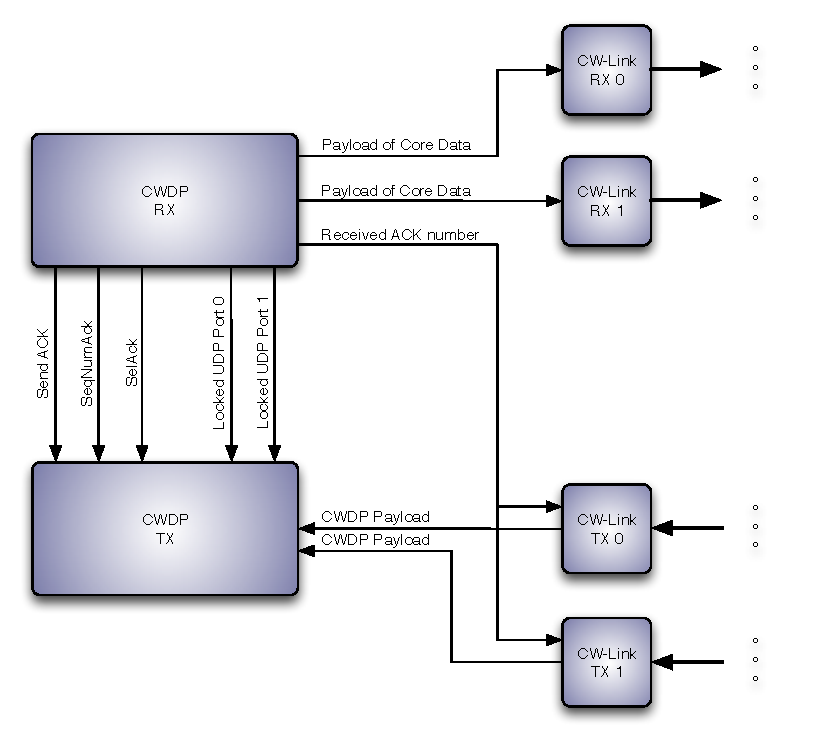
\includegraphics[scale=1,center]{Diagrams/CWDP-simplified-transaction-2.pdf}
  \caption{\ac{CWDP} Layer}\label{fig:CWDPSIMP2}
\end{figure}

\clearpage
\subsection{Arbiter}


% Esta secção tem de ser discutida e toda reformulada.
% porque é preciso dois estados stop e dois wait?
% precisas de uma tabela State | Description
% precisas de uma tabela Signal | Direction | Description 

To control the access to both the \ac{CWDP} TX and the RAM TX modules from the CW-Link TX modules an arbiter block has been implemented. The arbiter \ac{FSM} is described in Table \ref{table:Arbiter-FSM} (states), Table \ref{table:Arbiter Signals} (input/output signals), and Figure \ref{fig:arbiter} (state transition diagram). The arbiter's algorithm is simple and tries to ensure that both UDP ports get the same priority in using FaceWorks' transmission infrastructure: when both ports want to have access to the CWDP layer, control is toggled from the port that currently has control to the port that does not.

\begin{table}[h]
\centering
\caption{Arbiter FSM States}
\label{table:Arbiter-FSM}
\begin{tabular}{c l}
\hlinew{0.08cm}
\cellformatrG{}&
\cellformatlG{}
\\
\cellformatrG{\multirow{-2}{2cm}{\centering State}} &
\cellformatlG{\multirow{-2}{2cm}{\centering Description}}
\\
\hlinew{0.04cm}
\cellformatrW{ s\_stop }& 
Initial state. \ac{FSM} waits for a TX request from one of the Cw-Link units.
\\
\hlinew{0.04cm}
\cellformatrW{ s\_stop\_1 }& 
\ac{FSM} waits for a TX request from one of the Cw-Link units.
\\
\hlinew{0.04cm}
\cellformatrW{ s\_tx\_0 }& 
Resources Granted to Cw-Link 0.
\\
\hlinew{0.04cm}
\cellformatrW{ s\_tx\_1 }& 
Resources Granted to Cw-Link 1.
\\
\hlinew{0.04cm}
\cellformatrW{ s\_wait\_0 }& 
Waiting for Cw-Link 0 to free the Resources.
\\
\hlinew{0.04cm}
\cellformatrW{ s\_wait\_1 }& 
Waiting for Cw-Link 1 to free the Resources.
\\
\end{tabular}
\end{table}

\begin{table}[h]
\centering
\caption{Arbiter Input and Output Signals}
\label{table:Arbiter Signals}
\begin{tabular}{c c l}
\hlinew{0.08cm}
\cellformatrG{}&
\cellformatlrG{}&
\cellformatlG{}
\\
\cellformatrG{\multirow{-2}{2cm}{\centering Signals}} &
\cellformatlrG{\multirow{-2}{2cm}{\centering Direction}} &
\cellformatlG{\multirow{-2}{2cm}{\centering Description}}
\\
\hlinew{0.04cm}
\greyrow \multicolumn{3}{c}{CWDP}
\\
\hlinew{0.04cm}
\cellformatrW{ busy }& 
\cellformatlrW{ input }&
Signals that the \ac{CWDP} TX unit is being used.
\\
\hlinew{0.04cm}
\cellformatrW{ cwdp\_sent }& 
\cellformatlrW{ input }&
Signals that the packet was sent.
\\
%\multicolumn{3}{c}{\vspace*{-0.3cm}}\\
%%%%%%%%%%%%% SECOND PART OF THE TABLE %%%%%%%%%%%%%%%%%%%%%%%%
%\hlinew{0.08cm}
%\cellformatrG{}&
%\cellformatlrG{}&
%\cellformatlG{}
%\\
\hlinew{0.04cm}
\greyrow  \multicolumn{3}{c}{ CW-Link 0 }\\
\hlinew{0.04cm}
\cellformatrW{ active\_unit\_tx[0] }& 
\cellformatlrW{ output }&
Activates the CW-Link 0 unit.
\\
\hlinew{0.04cm}
\cellformatrW{ busy\_cwlink\_0 }& 
\cellformatlrW{ input}&
Signals that the CW-Link 0 is busy.
\\
\hlinew{0.04cm}
\cellformatrW{ cw\_req\_vector\_TX\_0 }& 
\cellformatlrW{ input }&
Signals that the Cw-Link 0 is requesting access.
\\
%\multicolumn{3}{c}{\vspace*{-0.3cm}}\\
%%%%%%%%%%%%% SECOND PART OF THE TABLE %%%%%%%%%%%%%%%%%%%%%%%%
%\hlinew{0.08cm}
%\cellformatrG{}&
%\cellformatlrG{}&
%\cellformatlG{}
%\\
\hlinew{0.04cm}
\greyrow  \multicolumn{3}{c}{ CW-Link 1 }\\
\hlinew{0.04cm}
\cellformatrW{ active\_unit\_tx[1] }& 
\cellformatlrW{ output }&
Activates the CW-Link 1 unit.
\\
\hlinew{0.04cm}
\cellformatrW{ busy\_cwlink\_1 }& 
\cellformatlrW{ input}&
Signals that the CW-Link 1 is busy.
\\
\hlinew{0.04cm}
\cellformatrW{ cw\_req\_vector\_TX\_1 }& 
\cellformatlrW{ input }&
Signals that the Cw-Link 1 is requesting access.
\\
\end{tabular}
\end{table}

\begin{figure}[h]
  \centering
      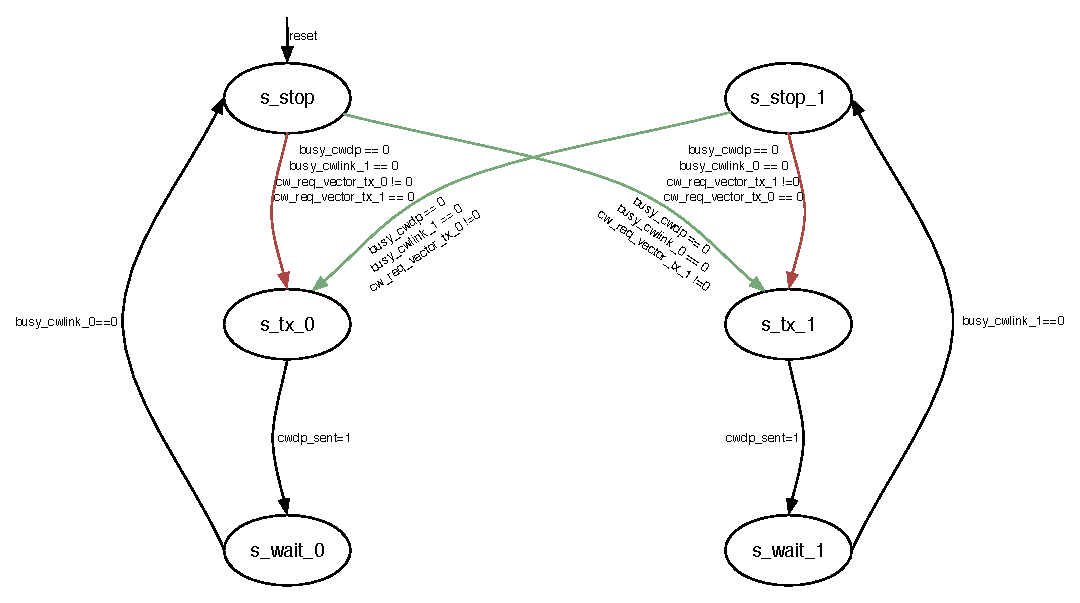
\includegraphics[scale=1,center]{Diagrams/arbiter-fsm.pdf}
  \caption{Arbiter \ac{FSM} State Transition Diagram}\label{fig:arbiter}
\end{figure}

%ainda nao meteste a indicaçao do estado inicial



% %%%%%%%%%%%%%%%%%%%%%%%%%%%%%%%%%%%%%%%%%%%%%%%%%%%%%%%%%%%%%%%%%%%%%%
% Your work: Chapter 4
% %%%%%%%%%%%%%%%%%%%%%%%%%%%%%%%%%%%%%%%%%%%%%%%%%%%%%%%%%%%%%%%%%%%%%%
\fancychapter{Verification}

In this chapter the methodology used to debug, verify and inspect the FaceWorks core is presented. 

Initially, verification of the design was being performed directly on the FPGA using as main tools for debug a packet sniffer (Wireshark), an \ac{ILA} (Xilinx's ChipScope Pro) and the Face-Test application to send stimuli to the FPGA board and analyze the responses. However, as the design got near completion, some intermittent bugs showed up, which were very difficult to identify using this ad-hoc verification method.

The main difficulty was to know when and what signal was the causing a problem, so that correct trigger conditions could be set. Using the ILA proved ineffective due to too many inconclusive trigger conditions, and a limited buffer size to store data samples for analysis, which is the result of having limited number of \acp{BRAM} in the device. 

An alternative consisted in creating a testbench and running the system into a simulator such Xilinx's iSim. However, it was difficult to recreate realistic test conditions, unless a significant amount of C and Verilog code were developed. Another way is to modify the system in order to be able to run a simpler to write testbench, but this approach is risky as important features may end up untested.

Besides, methods for the testbench to read and write data are limited to file \ac{IO} since no Verilog Procedural Interface (VPI) support is offered for iSim. Writing and reading files to exercise the MII interface in a testbench is hard and complicated to implement, considering the sheer amount of data needed to adequately test a network interface.  So other alternatives were searched so that the design could be properly debugged and verified. Of the considered alternatives, Verilator, a free open source application, has been chosen to perform this task.

This chapter describes Verilator, explaining C++ testbenchs, the process of instantiating Verilator generated SystemC models in C++ applications, and how to run simulations.


\section{Verilator}

Verilator is an application that translates a synthesizable Verilog description into an optimized cycle-accurate behavioral model in C++/SystemC, which is called a verilated file. Verilator is a two state simulator (0,1), but it has features to deal with unknown states. The testbench is a C/C++ application that wraps the verilated model and is compiled with it using a common C++ compiler. Verilated models show high simulation speed, which is on par or higher than commercial simulators such as NC-Verilog, VCS and others. \cite{veribench}.

\subsection{Verilator History}
Verilator was originally created in 1994 by Paul Wasson at the Core Logic Group at Digital Equipment Corporation (DEC). In 1998 DEC released the source of verilator under a GNU Public License. The maintainer of the project since 2001, Wilson Snyder, added SystemC support and fully rewrote Verilator in C++. Latest additions provide SystemVerilog and SystemVerilog Direct Programming Interface (DPI) language support\cite[p. 65]{verilatorman}.

\subsection{Verilator Testbench}

%Verificar a consistência de todos os títulos: se letras maisúcuilas são usadas então que seja em todos.

Using Verilator, a FaceWorks simulator has been created which can be stimulated with the same socket-based test application used for exercising FaceWorks in an FPGA. In this way test patterns that fail in the FPGA device can be replicated and analyzed in simulation with full visibility over all design signals. A FaceWorks SystemC model is created by running Verilator on the FaceWorks Verilog code, and this object is then instantiated in the testbench application.

\section{Verification Environment}


\begin{figure}[h]
  \centering
      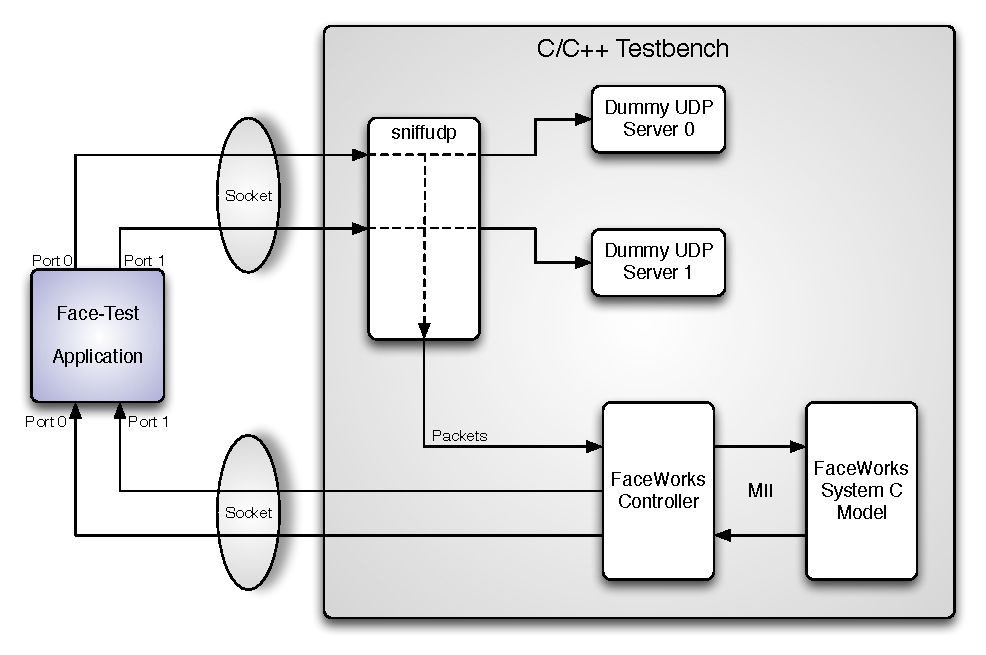
\includegraphics[scale=1,center]{Diagrams/TestBench-Diag.pdf}
  \caption{Verification Environment}\label{fig:tbschem}
\end{figure}


Figure \ref{fig:tbschem} shows the verification environment for FaceWorks, encompassing the Face-test application and the C++ testbench. The testbench has five components: 3 threads (\texttt{Dummy UDP Server 0}, \texttt{Dummy UDP Server 1} and {\tt sniffudp}), the FaceWorks Controller and the FaceWorks model.

The two threads \texttt{Dummy UDP Server 0} and \texttt{Dummy UDP Server 1} perform the simple operation of reading the \ac{UDP} ports persistently, so the input data coming from the application do not fill the OS socket buffer.

The {\tt sniffudp} thread launches the data capture code, which is based on the sniffex.c code example of {\tt libcap}, a portable C/C++ library for network traffic capture \cite{sniffer}. 

This data capture code must be used instead of a simple UDP socket, because this way the full Ethernet frame is captured, which makes it easier to reconstruct the MII packet in order to feed the data to the MII interface of the FaceWorks model.

The FaceWorks Controller is responsible for receiving data from the \texttt{sniffudp} thread, formatting the data according to the MII format and deliver them to the FaceWorks \ac{MII} interface. The FaceWorks Controller is also responsible for unpacking the data it receives from the FaceWorks model in order do send them to the test application via UDP sockets.

The FaceWorks model is a SystemC Model created by running Verilator on the FaceWorks Verilog code.

Threads are used so that the FaceWorks Controller can run at the same time as data is intercepted by the {\tt sniffudp} function. These two components are explained in detail in the next two subsections.


\subsection{sniffudp}

A simpler solution to capture data from the Face-Test application is to implement a C/C++ \ac{UDP} socket server in the testbench to read the incoming data from the Face-Test application and provide it to the FaceWorks SystemC model. However, since the FaceWorks connection to the outside is the \ac{MII} interface, one would need to recreate the MII packet from the received \ac{UDP} payload. Recreating the MII packet implies recreating the UDP packet followed by the \ac{IP} packet, followed the Ethernet frame. This would be unnecessarily complicated.

A solution for this problem is to capture the packets at the data link layer, which can be accomplish by the use of \texttt{libpcap}, avoiding the process of recreating the Ethernet, \ac{IP} and \ac{UDP} packets.

The \texttt{sniffudp} function is set to capture data on the Linux loopback ({\tt lo}) device, which are addressed with the two FaceWorks \ac{UDP} ports. The {\tt lo} device is a virtual network interface used to receive packets sent from the host to itself. After the setup the \texttt{sniffudp} thread blocks waiting for filtered packets. When such packets arrive they are passed to a callback function \texttt{got\_packet()}.

The \texttt{got\_packet()} function receives almost complete Ethernet frames (Figure \ref{fig:Eth-frame}) which miss the \ac{FCS} field and have a blank destination and source address, since the data is traveling through the loopback interface. The fields preamble, \ac{SFD}, destination address, source address and Ethertype are inserted. The data field (containing the \ac{IP} packet) is copied from the sniffed packet. The \ac{CRC} is calculated as described in section \ref{subsec:CRC} and appended as the FCS field.

Then, the \texttt{got\_packet()} function reaches a critical region where it pushes the packet into a queue shared with the main thread, after which it terminates execution. When another packet is filtered the callback function is called again and the process repeats all over again.


\subsection{FaceWorks Controller}

The FaceWorks Controller instantiates the FaceWorks model, and communicates with it. The communication with the model is presented in this section, and the instantiation of the model is presented in \ref{sec:vermodinst}.

Since the FaceWorks Controller does not implement the \ac{ARP} protocol, to properly support the communication between the Face-Test application and the FaceWorks model, the FaceWorks controller starts by sending a fixed \ac{ARP} reply packet as shown in Figure \ref{fig:Arp-packet}. This packet is sent even without receiving any \ac{ARP} request from the FaceWorks model. The purpose is to fill the \ac{ARP} cache with an IP address / \ac{MAC} address pair, so the FaceWorks Ethernet TX module can obtain the MAC address  by consulting the \ac{ARP} module. If the cache is already stuffed, no \ac{ARP} query packets will be generated by the FaceWorks model.

\begin{figure}[h]
  \centering
      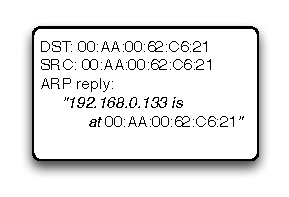
\includegraphics[scale=1,center]{Diagrams/ARP-stuffing.pdf}
  \caption{Injected \ac{ARP} Reply Packet }\label{fig:Arp-packet}
\end{figure}

After the \ac{ARP} stuffing is completed, the FaceWorks controller is in a loop, trying to transfer data from the packet queue, shared with the \texttt{sniffudp} thread, to the \ac{MII} RX interface of the FaceWorks model, and/or to transfer data from the \ac{MII} TX interface to the socket that leads to the Face-Test application.

To transfer data from the queue to the MII RX interface the FaceWorks controller needs to get hold of the mutex that protects the shared packet queue. When access to the mutex is granted and at least one packet exists in the queue, the packet is popped from the queue and fed into the \ac{MII} RX interface of the FaceWorks model, nibble by nibble.

To transfer data to the socket leading to Face-Test, the FaceWorks controller  stores the received nibbles in a buffer, which is then passed to another function, the \texttt{process\_recv\_packet} function discussed in the next section, which verifies and forwards the data to the Face-Test application.


\subsection{process\_recv\_packet}
\label{subsec:process_recv}

The \texttt{process\_recv\_packet} function receives as argument a packet buffer from the FaceWorks controller, processes the packet and sends it over the network socket to the Face-Test application.

The \texttt{process\_recv\_packet} function checks if the Preamble, \ac{SFD} and Ethernet headers are correctly constructed, by comparing their values to the expected values. The \ac{FCS} field is calculated for the received packet and compared with the \ac{FCS} value in the packet itself. The FCS field contains a \ac{CRC} checksum computed as described in section \ref{subsec:CRC}. If any field does not match the expected value, the function returns with an error which indicates the malformed field.

If a well formed packet is received, the \ac{IP} headers and \ac{UDP} headers are read to extract the destination \ac{IP} address, \ac{UDP} port and \ac{UDP} payload offset, and the \ac{UDP} packet is sent to the Face-Test Application.

By verifying the data from the \ac{MII} interface, the operation of the FaceWorks model is always under scrutiny, which is a valuable debug feature. Next, the Ethernet, \ac{IP} and \ac{UDP} headers are removed,  and the data is placed into the \ac{UDP} socket to be sent to the Face-Test application, which is listening to the UDP ports in use.


\subsection{Cyclic Redundancy Check}
\label{subsec:CRC}
The \ac{CRC} is computed by both the \texttt{process\_recv\_packet} and the \texttt{got\_packet} function. The source code used to calculate the \ac{CRC} has been generated by a Python script denominated \texttt{pycrc}\cite{pycrc}. The \texttt{pycrc} script outputs  a C header file (.h) and C source code file (.c) which can compute the CRC. 

\begin{figure}[h]
\begin{boxedverbatim}
> python pycrc.py --model crc-32 --algorithm table-driven --poly 0x04c11db7 --generate h -o crc.h

> python pycrc.py --model crc-32 --algorithm table-driven --poly 0x04c11db7 --generate c -o crc.c
\end{boxedverbatim}
\caption{Generating \ac{CRC} Functions with the {\tt pycrc} Python Script}
\label{chp4:crcgen}
\end{figure}

Figure \ref{chp4:crcgen} illustrates how to use the \texttt{pycrc} script. The script must be called twice: the first time to generate the .h file and the second time to generate the .c file. The command line arguments provided are the appropriate ones to generate the Ethernet \ac{FCS}, a 32-bit CRC which uses the 0x04c11db7 polynomial. The {\tt -algorithm table-driven} option has been included because it produces the fastest algorithm. This method uses a look-up table which might not be acceptable for embedded systems. But, since this is only used in the testbench program which runs on the PC, memory restrictions do not apply.


\section{Verilator Module Instantiation}
\label{sec:vermodinst}
The Verilog module declaration of the FaceWorks system is depicted in Figure \ref{chp4:fawsystem}. The testbench code has been written based on the {\tt test\_sc} and {\tt test\_sp} examples included as part of the Verilator installation directory {\tt ~verilator/examples/} \cite{verilatorman}.

\begin{figure}[h]
\begin{boxedverbatim}
module faw_system(
        input wire sys_clk,
        input wire sys_rst,
        //!IP/PORT CONFIG PINS
        input wire[3:0] faw_dyn_conf,
        input wire faw_sub_net,
   
        //!ETHERNET PHY PINS  
        input wire MAC_PHY_tx_clk_pin;
        input wire MAC_PHY_rx_clk_pin;
        input wire MAC_PHY_rx_dv_pin;
        input wire [3:0] MAC_PHY_rx_data_pin;
        output wire MAC_PHY_tx_en_pin;
        output wire MAC_PHY_tx_error_pin;
        output wire [3:0] MAC_PHY_tx_data_pin;
        output wire MAC_PHY_rst_n;
        output wire MAC_PHY_mdc;
);

\end{boxedverbatim}
\caption{FaceWorks Verilog Module Declaration (faw\_system.v)}
\label{chp4:fawsystem}
\end{figure}

In the testbench code quite a few declarations are needed to instantiate the FaceWorks verilated model. For this it is necessary to include the following header files, as shown in Figure \ref{chp4:fawheader}.

\begin{figure}[h]
\begin{boxedverbatim}
#ifdef SYSTEMPERL
# include "systemperl.h"	// SystemC + SystemPerl global header
# include "sp_log.h"		// Logging cout to files
# include "SpTraceVcd.h"
# include "SpCoverage.h"
#else
# include "systemc.h"		// SystemC global header
# include "verilated_vcd_sc.h"	// Tracing
#endif

#include "Vfaw_system.h" // Top level header, generated from verilator

\end{boxedverbatim}
\caption{Testbench Header Files}
\label{chp4:fawheader}
\end{figure}

The testbench code supports two type of simulations: the SystemC simulation (signal tracing) and the SystemC + SystemPerl simulation (code coverage and signal tracing). The \#ifdef clause in Figure \ref{chp4:fawheader} selects the correct header files depending on the simulation case. Then the header file Vfaw\_system.h, which results from running Verilator run on the FaceWorks Verilog code, is included.

\begin{figure}[h]
\begin{boxedverbatim}

int sc_main(int argc, char* argv[]) {
(...)
    //
    // Define the Clocks
    //
#if (SYSTEMC_VERSION>=20070314)
	sc_clock sys_clk     ("sys_clk", 20,SC_NS, 0.5,10,SC_NS, false);
	sc_clock MAC_PHY_tx_clk_pin     ("MAC_PHY_tx_clk_pin", 40, SC_NS, 0.5, 0, SC_NS, false);
	sc_clock MAC_PHY_rx_clk_pin     ("MAC_PHY_rx_clk_pin", 40, SC_NS, 0.5, 0, SC_NS, false);
#else
	sc_clock sys_clk     ("sys_clk", 20, 0.5, 10, false);
	sc_clock MAC_PHY_tx_clk_pin     ("MAC_PHY_tx_clk_pin", 40, 0.5, 0, false);
	sc_clock MAC_PHY_rx_clk_pin     ("MAC_PHY_rx_clk_pin", 40, 0.5, 0, false);
#endif

	//==========
	// Define the Interconnect
	cout << "Defining Interconnect\n";
	sc_signal<bool> sys_rst;
	sc_signal<vluint32_t > faw_dyn_conf;
	sc_signal<bool > faw_sub_net;
	sc_signal<bool> MAC_PHY_tx_en_pin;
	sc_signal<bool> MAC_PHY_tx_error_pin;
	sc_signal<vluint32_t> MAC_PHY_tx_data_pin;
	sc_signal<bool> MAC_PHY_rx_dv_pin;
	sc_signal<vluint32_t > MAC_PHY_rx_data_pin;
	sc_signal<bool> MAC_PHY_rst_n;
	sc_signal<bool> MAC_PHY_mdc;
\end{boxedverbatim}
\caption{Signal Declaration in the SystemC Testbench}
\label{chp4:faw_signal_decl}
\end{figure}

The testbench is written in SystemC and therefore the main function is denoted {\tt sc\_main}, as shown in Figure \ref{chp4:faw_signal_decl}.

% mete os \tt
To declare the SystemC clock and signal objects, the \texttt{sc\_clock} and \texttt{sc\_signal} classes are used.
The \texttt{sys\_clk} object is a clock with a period of 20 ns (SC\_NS is used to specify time units), a duty cycle of 50\%, the first transition occurs at 10 ns, and is a negative edge transition ({\tt false}). This signal drives the FaceWorks clock pin. The other two clock signals, {\tt(MAC\_PHY\_tx\_clk\_pin} and  {\tt MAC\_PHY\_rx\_clk\_pin)}, are used in the \ac{MII}/\ac{MAC} interface, and have similar declarations.

For the rest of the signals (ie, signals that are not clocks), the {\tt sc\_signal} class is used, which declares signals of various data types. Single bit signals use the {\tt bool} type, 2 to 32-bit vectors use the {\tt vluint32\_t} type, 33 to 64-bit vectors  use the {\tt  vluint64\_t} or the { \tt sc\_bv} types\footnote{The sc\_bv is also used for 33 to 64-bit vectors if the -no-pins64 flag is provided to Verilator}, and wider bit vectors use the {\tt sc\_bv} type. When Verilator translates Verilog code to SystemC, the {\tt  SC\_MODULE} pinout will show the type conversions described, as can be seen in the output header file Vfaw\_system.h, where only \texttt{bool} and  \texttt{vluint32\_t} types are used. The reasons for these type conversions are linked with the simulator's performance.

\begin{figure}[H]
\begin{boxedverbatim}
	//==========
	// Device under test
#ifdef SYSTEMPERL
	SP_CELL (top, Vfaw_system);
	SP_PIN (top, sys_clk,sys_clk);
	SP_PIN (top, MAC_PHY_tx_clk_pin,MAC_PHY_tx_clk_pin);
	SP_PIN (top, MAC_PHY_rx_clk_pin,MAC_PHY_rx_clk_pin);
	SP_PIN (top, sys_rst,	sys_rst);
	SP_PIN (top, faw_dyn_conf,	faw_dyn_conf);
	SP_PIN (top, faw_sub_net,	faw_sub_net);
	SP_PIN (top, MAC_PHY_tx_en_pin,	MAC_PHY_tx_en_pin);
	SP_PIN (top, MAC_PHY_tx_error_pin,	MAC_PHY_tx_error_pin);
	SP_PIN (top, MAC_PHY_tx_data_pin,	MAC_PHY_tx_data_pin);
	SP_PIN (top, MAC_PHY_rx_dv_pin,	MAC_PHY_rx_dv_pin);
	SP_PIN (top, MAC_PHY_rx_data_pin,	MAC_PHY_rx_data_pin);
	SP_PIN (top, MAC_PHY_rst_n,	MAC_PHY_rst_n);
	SP_PIN (top, MAC_PHY_mdc,	MAC_PHY_mdc);
#else
	Vfaw_system* top = new Vfaw_system("top");
	top->sys_clk		(sys_clk);
	top->MAC_PHY_tx_clk_pin	        (MAC_PHY_tx_clk_pin);
	top->MAC_PHY_rx_clk_pin		(MAC_PHY_rx_clk_pin);
	top->sys_rst	(sys_rst);
	top->faw_dyn_conf	(faw_dyn_conf);
	top->faw_sub_net	(faw_sub_net);
	top->MAC_PHY_tx_en_pin	        (MAC_PHY_tx_en_pin);
	top->MAC_PHY_tx_error_pin		(MAC_PHY_tx_error_pin);
	top->MAC_PHY_tx_data_pin	(MAC_PHY_tx_data_pin);
	top->MAC_PHY_rx_dv_pin	(MAC_PHY_rx_dv_pin);
	top->MAC_PHY_rx_data_pin	(MAC_PHY_rx_data_pin);
	top->MAC_PHY_rst_n	(MAC_PHY_rst_n);
	top->MAC_PHY_mdc	(MAC_PHY_mdc);
#endif

\end{boxedverbatim}
\caption{Interconnecting the Verilated Model and the Testbench Signals}
\label{chp4:faw_signal_interc}
\end{figure}

After all signals are declared, they are used to connect the testbench signals to the Verilator module pins. Another \#ifdef clause is used to select if the verilated module is instantiated using SystemPerl or SystemC, as show in Figure \ref{chp4:faw_signal_interc}. With the SystemC model instantiated and the signals connected in the C++ testbench,  the model is ready to be initialized and run.
\clearpage


\section{Running the Simulation Model}

To ease the compiling and running of the simulation model, two different Makefile sets have been created. One set of makefiles generates the SystemC model and runs the simulation to produce wave traces. The other set of Makefiles creates the SystemC and SystemPerl code to produce wave traces and coverage metrics.

\subsection{Folder Structure}

In Figure \ref{fig:foldhier}, a representation of the folder structure used for the project is shown. Each folder is explained as follows:

\begin{itemize}
\item faw\_sys\_verilog: contains the Verilog source of FaceWorks;
\item test\_sc: contains the Makefiles and the testbench source code for generating the SystemC simulation;
\item test\_sp: contains the makefiles for the SystemC/SystemPerl simulation;
\item src: contains files that are used as input to verilator.
\end{itemize}

\begin{figure}[h]
  \centering
      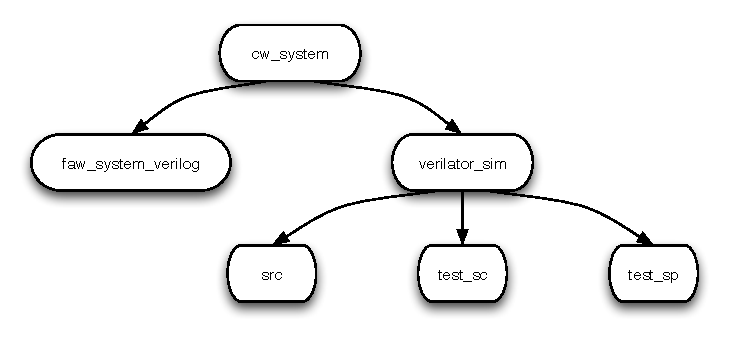
\includegraphics[scale=0.75]{Diagrams/Pastas.pdf}
  \caption{Project Folder Hierarchy}\label{fig:foldhier}
\end{figure}

\subsection{Producing the Simulation Model} 
The SystemC simulation model is produced by the Makefile in the test\_sc folder, which starts by invoking Verilator, as shown in Figure \ref{fig:veriflagstrace}, with the following flags:
\begin{itemize}
\item --sc: generates SystemC output;
\item -f: specifies an input file with commands;
\item --trace: produces waveform traces while running.
\end{itemize}

\begin{figure}[h]
\begin{boxedverbatim}
verilator --sc -f ../src/input.vc faw_system.v --trace
\end{boxedverbatim}
\caption{Verilator Invocation}
\label{fig:veriflagstrace}
\end{figure}

The Verilator input file {\tt input.vc} placed in the src folder is shown in Figure \ref{fig:inputfile}. The {\tt input.vc} file contains directives for file extensions and directories where the Verilog sources can be found.

\begin{figure}[h]
\begin{boxedverbatim}
+librescan +libext+.v
+incdir+../../faw_sys_verilog
\end{boxedverbatim}
\caption{Verilator Directives}
\label{fig:inputfile}
\end{figure}

After the input files are verilated the Makefile will call the Makefile\_obj file to compile the testbench source code and link it with the verilated model.

The resulting application needs to capture network packets without running in super-user mode. This is accomplished by specific Linux settings and by using the {\tt setcap} application. The makefile automatically makes these settings and runs the simulator application.

\subsection{Linting the Verilog Code}

When executing, Verilator first verifies if lint violations exist, to ensure the code is synthesizable. If any warning or error exists in the code Verilator aborts execution unless the particular line of code causing the error or warning is protected with a pair of pragmas, as depicted in Figure \ref{fig:lintdisable}.

\begin{figure}[h]
\begin{boxedverbatim}
/*verilator lint_off PINNOCONNECT*/
.crcValid(/* open */),
/*verilator lint_on PINNOCONNECT*/
\end{boxedverbatim}
\caption{A Linting Warning Disabled}
\label{fig:lintdisable}
\end{figure}

Warnings can be ignored by calling verilator with the flag -Wno-warning. Verilator may also be used exclusively as a "linting" tool, invoking Verilator with the flag --lint-only.
Some of the warnings/errors produced by Verilator can have an impact on the performance of the model and produce non-synthesizable code; so it is recommended to correct all linting warnings before proceeding. Some examples of the verilator warnings that occurred while processing FaceWorks are illustrated below. For each one of these warnings the problem was identified and solved.
\clearpage

In Figure \ref{fig:casewarn}, the Case Overlap and Case Incomplete warnings produced by a {\tt case} statement were due to a user error in the Verilog description. One of the case values overlaps the case value (0x4), and leaves the case value 0x07 uncovered, as no default case statement is given.

\begin{figure}[h]
\begin{boxedverbatim}
%Warning-CASEOVERLAP: ../../faw_sys_verilog/faw_cwdp_rx.v:571:
Case values overlap (example pattern 0x4)
%Warning-CASEOVERLAP:
Use "/* verilator lint_off CASEOVERLAP */" and lint_on around source to disable this message.
%Warning-CASEINCOMPLETE: ../../faw_sys_verilog/faw_cwdp_rx.v:555:
Case values incompletely covered (example pattern 0x7)
\end{boxedverbatim}
\caption{Case Overlap and Case Incomplete Warnings}
\label{fig:casewarn}
\end{figure}

This specific situation, which was caused by a typo, is easy to correct by changing the value of the overlapping statement to the expected value, fixing both warnings. In other cases, where a full coverage of input signal combinations is not obtained, one needs to insert the {\tt default} statement, so that the warning does not display.
\vspace{0.5cm}

In Figure \ref{fig:addsmallerrightside}, the 11-bit signal {\tt CWDP\_data\_size} is added to the 4-bit constant in the \ac{RHS} of the expression. Although this is a valid Verilog expression, and accepted by tools such as \ac{XST}, this code produces the Verilator warning depicted in Figure \ref{fig:casewidth}.

\begin{figure}[h]
\begin{boxedverbatim}
packet_size_next = CWDP_data_size + 4'h 4;
\end{boxedverbatim}
\caption{Addition with Narrower \acs{RHS} Warning}
\label{fig:addsmallerrightside}
\end{figure}

\begin{figure}[h]
\begin{boxedverbatim}
%Warning-WIDTH: ../../faw_sys_verilog/faw_cwdp_tx.v:255:
Operator ADD expects 11 bits on the RHS, but RHS's CONST '4'h4' generates 4 bits.
%Warning-WIDTH: 
Use "/* verilator lint_off WIDTH */" and lint_on around source to disable this message.
\end{boxedverbatim}
\caption{Width Mismatch Warning}
\label{fig:casewidth}
\end{figure}

To solve the Width Mismatch warning, the missing \acp{MSB} on the \ac{RHS} of the expression must be declared as depicted in Figure \ref{fig:casewidthsolve}. This way the two operands and the sum are 11-bit vectors. A 12-bit vector for the sum would also be acceptable.

\begin{figure}[H]
\begin{boxedverbatim}
packet_size_next = CWDP_data_size + {7'b0,4'h 4};
\end{boxedverbatim}
\caption{Correction of the Previous Width Mismatch Problem}
\label{fig:casewidthsolve}
\end{figure}

\clearpage

The warning presented in Figure \ref{fig:unoptflatwarn} identifies a path that contains circular logic. It is unlikely that the resulting asynchronous logic will meet the desired functionality. Also, this may affect the Verilator model performance, so it is recommended to fix this problem.

\begin{figure}[h]
\begin{boxedverbatim}
%Warning-UNOPTFLAT: ../../faw_sys_verilog/faw_faceworks.v:302:
Signal unoptimizable: Feedback to clock or circular logic: v.facework.active_unit_tx
%Warning-UNOPTFLAT: Example path: ../../faw_sys_verilog/faw_faceworks.v:302:  v.facework.active_unit_tx
%Warning-UNOPTFLAT: Example path: ../../faw_sys_verilog/faw_faceworks.v:749:  ASSIGNW
%Warning-UNOPTFLAT: Example path: ../../faw_sys_verilog/faw_faceworks.v:270:  v.facework.CWDP_nr
%Warning-UNOPTFLAT: Example path: ../../faw_sys_verilog/faw_cwdp_tx.v:175:  ALWAYS
%Warning-UNOPTFLAT: Example path: ../../faw_sys_verilog/faw_faceworks.v:357:  v.facework.busy_cwdp
%Warning-UNOPTFLAT: Example path: ../../faw_sys_verilog/faw_faceworks.v:681:  ALWAYS
%Warning-UNOPTFLAT: Example path: ../../faw_sys_verilog/faw_faceworks.v:302:  v.facework.active_unit_tx
%Error: Exiting due to 2 warning(s)
%Error: Command Failed /usr/local/bin/verilator_bin --sc -f ../src/input.vc faw_system.v --trace
\end{boxedverbatim}
\caption{Circular Logic Warning}
\label{fig:unoptflatwarn}
\end{figure}

As one can see in Figure \ref{fig:unoptflatwarn}, the combinatorial loop starts and ends in the signal {\tt active\_unit\_tx}. This warning is corrected by changing the assignments done to the \texttt{active\_unit\_tx} signal within the \ac{FSM} to break the existing feedback loop.


\subsection{Observing Wave Traces}

Assuming no warning or errors were detected during the lint and compile phases, the simulator model is run and the Face-Test application stimulates it. After a predefined number of exchanged packets, the simulator terminates execution and dumps a VCD file that contains the simulation waveforms.

To display the contents of the VCD file, the Makefile launches the GTKwave application \cite{gtkwave}. With GTKWave the full hierarchy of the design is shown, and the desired signals or registers can be added to the visualization window. In Appendix \ref{Appendix A}, a screen shot showing the GTKwave application can be seen.


\subsection{Coverage}

To generate coverage metrics the SystemPerl Makefile inside the {\tt test\_sp} folder must be used. This causes a coverage file name {\tt coverage.pl} to be written in the {verilator\_sim/test\_sp/logs/} folder when the simulation ends. Naturally, coverage results depend on the quality of the stimulus provided by the Face-Test application.
\clearpage
The application Vcoverage, part of the SystemPerl toolkit, can output a copy of the source code files of the project with coverage metrics annotated. By default, the file {\tt logs/coverage.pl} is read to annotate the source code and place a copy under {logs/coverage\_source/} , as shown in Figure \ref{fig:vcov_outp}.

\begin{figure}[h]
\begin{boxedverbatim}
> vcoverage
Total coverage (398/687) 57.93%
See lines with '\%00' in logs/coverage\_source
\end{boxedverbatim}
\caption{Output from Vcoverage}
\label{fig:vcov_outp}
\end{figure}

For different stimulus patterns, distinct output coverage files are obtained. To combine these into a single coverage file the {\tt vcoverage} application is called with the arguments presented in Figure \ref{fig:vcov_join}.

\begin{figure}[h]
\begin{boxedverbatim}
> vcoverage --noreport -write logs/merged-cov.dat *.pl
Generating the report
> vcoverage --min 1 --o logs/coverage_source logs/merged-cov.dat 
Total coverage (524/687) 76.27%
See lines with '\%00' in logs/coverage\_source
\end{boxedverbatim}
\caption{Merging Distinct Coverage Files and Generating Output Statistics}
\label{fig:vcov_join}
\end{figure}

First, all {\tt .pl} files are merged into a single {\tt merged-cov.dat} file by using the --noreport option. Then, coverage statistics are generated for the joined files and the output source code files are placed in the same output directory {\tt logs/coverage\_source}.

\begin{figure}[h]
\begin{boxedverbatim}
014988		s_wait_1 : begin
 000026		   if((busy_cwlink_1 == 1'b 0)) begin
		      // Ack foi recebido
		      active_unit_tx_next=2'b 00;
		      next_state = s_stop_1;
		   end
		end
	
%000000		default: begin
	 	   active_unit_tx_next = 2'b 00;
		   next_state = s_stop;
		end
\end{boxedverbatim}
\caption{Code Coverage Report Excerpt}
\label{fig:cov_ex}
\end{figure}

As shown in the Verilog code example in Figure \ref{fig:cov_ex}, the number of times each code block is executed is annotated on the left. Code that {\tt vcoverage} thinks needs more coverage is marked \% X, where X is the number of times the line has been exercised. Any line exercised less than a minimum number of times (which can be specified with the {\tt --min} option) is marked \% X.

% Ensure that the next chapter starts in a odd page
\cleardoublepage




% %%%%%%%%%%%%%%%%%%%%%%%%%%%%%%%%%%%%%%%%%%%%%%%%%%%%%%%%%%%%%%%%%%%%%%
% Conclusions
% %%%%%%%%%%%%%%%%%%%%%%%%%%%%%%%%%%%%%%%%%%%%%%%%%%%%%%%%%%%%%%%%%%%%%%
\fancychapter{Results}

In this chapter two kind of results are presented: 1) FPGA implementation results on consumed resources and operation frequency; 2) bandwidth results. 

\section{FPGA Implementation Results}

The system has been developed and tested on a Xilinx SP605 board, featuring a Spartan 6 XC6SLX45T device and a Marvell Alaska PHY (88E1111) chip. The Spartan 6 is a low end device, designed for larger production volumes and low price but with limited performance.

The synthesis results presented are obtained with the Xilinx ISE 14.4 suite of tools. In Table \ref{table:Implementation Results of the single port FaceWorks}, synthesis results for the original single port implementation are presented. Table \ref{table:Implementation Results of the two port FaceWorks} presents synthesis results for the two-port implementation designed in this work.

\begin{table}[h]
\centering
\caption{Implementation Results for the Single-Port FaceWorks}
\label{table:Implementation Results of the single port FaceWorks}
\begin{tabular}{c c c c}
\hlinew{0.08cm}
\cellformatrG{}&\cellformatlrG{}&\cellformatlrG{}&\cellformatlG{}\\
\cellformatrG{\multirow{-2}{7 cm}{}} &
\cellformatlrG{\multirow{-2}{2cm}{\centering Used}}&
\cellformatlrG{\multirow{-2}{1.8cm}{\centering Total}}&
\cellformatlG{\multirow{-2}{2cm}{\centering Percentage Used}}
\\
\hlinew{0.08cm}
\greyrow \multicolumn{4}{c}{Slice Logic Utilization}
\\
\hlinew{0.04cm}
\cellformatrW{\-\hspace{0.5cm}Number of Slice Registers\hfill } & \cellformatlrW{1527} & \cellformatlrW{54576} & \cellformatlW{2\%}\\
\cellformatrW{Number of Slice LUTs:\hfill} & \cellformatlrW{2178} & \cellformatlrW{27288} & \cellformatlW{7\%}\\
\cellformatrW{\hfill Number used as Logic} & \cellformatlrW{2036} & \cellformatlrW{27288} & \cellformatlW{7 \%}\\
\cellformatrW{\hfill \-\hspace{1.5cm}Number used as Memory} & \cellformatlrW{16} & \cellformatlrW{6048} & \cellformatlW{1 \%}\\
\hlinew{0.08cm}
\greyrow \multicolumn{4}{c}{Slice Logic Distribution}
\\
\hlinew{0.04cm}
\cellformatrW{Number of LUT Flip Flop pairs used:\hfill } & \cellformatlrW{2375} & \cellformatlrW{-} & \cellformatlW{-}\\
\cellformatrW{\-\hspace{2cm}Number with an unused Flip Flop} & \cellformatlrW{999} & \cellformatlrW{2375} & \cellformatlW{42\%}\\
\cellformatrW{\-\hspace{1.3cm}Number with an unused LUT\hfill} & \cellformatlrW{197} & \cellformatlrW{2375} & \cellformatlW{8 \%}\\
\cellformatrW{\-\hspace{2.2cm}Number of fully used LUT-FF pairs\hfill} & \cellformatlrW{1179} & \cellformatlrW{2375} & \cellformatlW{49 \%}\\
\hlinew{0.08cm}
\greyrow \multicolumn{4}{c}{Specific Feature Utilization}
\\
\hlinew{0.04cm}
\cellformatrW{Number of Block RAM (16Kb)} & \cellformatlrW{2} & \cellformatlrW{116} & \cellformatlW{2\%}\\
\hlinew{0.08cm}


\end{tabular}
\end{table}



\begin{table}[h]
\centering
\caption{Implementation Results for the Two-Port FaceWorks}
\label{table:Implementation Results of the two port FaceWorks}
\begin{tabular}{c c c c}
\hlinew{0.08cm}
\cellformatrG{}&\cellformatlrG{}&\cellformatlrG{}&\cellformatlG{}\\
\cellformatrG{\multirow{-2}{7 cm}{}} &
\cellformatlrG{\multirow{-2}{2cm}{\centering Used}}&
\cellformatlrG{\multirow{-2}{1.8cm}{\centering Total}}&
\cellformatlG{\multirow{-2}{2cm}{\centering Percentage Used}}
\\
\hlinew{0.08cm}
\greyrow \multicolumn{4}{c}{Slice Logic Utilization}
\\
\hlinew{0.04cm}
\cellformatrW{\-\hspace{0.5cm}Number of Slice Registers\hfill } & \cellformatlrW{1917} & \cellformatlrW{54576} & \cellformatlW{3\%}\\
\cellformatrW{Number of Slice LUTs:\hfill} & \cellformatlrW{2965} & \cellformatlrW{27288} & \cellformatlW{10\%}\\
\cellformatrW{\hfill Number used as Logic} & \cellformatlrW{2933} & \cellformatlrW{27288} & \cellformatlW{10 \%}\\
\cellformatrW{\hfill \-\hspace{1.5cm}Number used as Memory} & \cellformatlrW{32} & \cellformatlrW{6048} & \cellformatlW{1 \%}\\
\hlinew{0.08cm}
\greyrow \multicolumn{4}{c}{Slice Logic Distribution}
\\
\hlinew{0.04cm}
\cellformatrW{Number of LUT Flip Flop pairs used:\hfill } & \cellformatlrW{3963} & \cellformatlrW{-} & \cellformatlW{-}\\
\cellformatrW{\-\hspace{2cm}Number with an unused Flip Flop} & \cellformatlrW{2046} & \cellformatlrW{3963} & \cellformatlW{51\%}\\
\cellformatrW{\-\hspace{1.3cm}Number with an unused LUT\hfill} & \cellformatlrW{998} & \cellformatlrW{3963} & \cellformatlW{25 \%}\\
\cellformatrW{\-\hspace{2.2cm}Number of fully used LUT-FF pairs\hfill} & \cellformatlrW{919} & \cellformatlrW{3963} & \cellformatlW{23 \%}\\
\hlinew{0.08cm}
\greyrow \multicolumn{4}{c}{Specific Feature Utilization}
\\
\hlinew{0.04cm}
\cellformatrW{Number of Block RAM (16Kb)} & \cellformatlrW{3} & \cellformatlrW{116} & \cellformatlW{2\%}\\
\hlinew{0.08cm}


\end{tabular}
\end{table}



\clearpage
The synthesis results show that both FaceWorks designs are very economic in terms of size. The single-port design uses the equivalent of 14000 gates, while the two-port design uses about 20000 gates\footnote{This figure has been obtained by counting 6 gates per each 6-input LUT and one gate per flip-flop}. However, it must be noted that the single-port design only supports 8 CW-Link connections, while the two-port design supports 16 CW-Link connections. The IP cores use very little memory and zero DSP blocks. The overall size can be considered adequate for a test and debug core. For a small FPGA like the Spartan 6 , it only occupies 10 \% of the logic resources in the two-port configuration. 

The results show that with about 7000 gates  a new UDP port and 8 new CW-Link connections can be added to the design. Thus, the design scales almost linearly, being the non-linear part the small amount of logic needed to augment the size of the arbiter.

\begin{table}[h]
\centering
\caption{Period Timing Constraints}
\label{table:Timing Constratints of the Dual Port FaceWorks}
\begin{tabular}{c c c}
\hlinew{0.08cm}
\cellformatrG{}&\cellformatlrG{}&\cellformatlG{}\\
\cellformatrG{\multirow{-2}{*}{\centering }} &
\cellformatlrG{\multirow{-2}{2cm}{\centering Used}}&
\cellformatlG{\multirow{-2}{1.8cm}{\centering Minimum}}
\\
\hlinew{0.04cm}
\cellformatrW{ Sys\_clk } & \cellformatlrW{20 ns} & \cellformatlW{8.341 ns}\\
\cellformatrW{ TX\_CLK } & \cellformatlrW{40 ns} & \cellformatlW{ NA }\\
\cellformatrW{ RX\_CLK } & \cellformatlrW{40 ns} & \cellformatlW{ NA }\\
\end{tabular}
\end{table}

The system clock period used and the minimum period constraint that has been possible to meet are shown in Table  \ref{table:Timing Constratints of the Dual Port FaceWorks}. The minimum period (8.341 ns), which corresponds to about 120MHz is a competitive frequency for a Spartan 6 device. Compared to the single port implementation, where the minimum clock period is 6.912 ns, the minimum clock period increases 20\% for the two-port implementation. This is mostly due the Arbiter block design, which scales poorly in terms of frequency. A better design would not be very difficult to implement but falls out of the scope of this thesis.  For a number of ports higher than two, it is highly recommended that the Arbiter design is reviewed.

\section{Ethernet Switch Characterization}

The results presented in this thesis have been obtained on a notebook with an Intel U4100 @ 1.30GHz processor, 3 GB of RAM and an Atheros AR8131 ethernet adapter, running the Linux kernel 3.2.0-x86-64. To interconnect Ethernet devices a TP-Link TL-WR841N switch has been used. Two network tests have been performed to the determine the switch capabilities, and detect if in either case they could limit the FaceWorks performance.

The first test was designed to determine the maximum throughput achievable with the switch. This test  consisted in exchanging data in both directions, simultaneously, between two notebooks interconnected via the switch. To establish the network connections between the notebooks the {\tt netcat (nc)} application was used in \ac{UDP} mode. To avoid limitations in hard disk throughput, the outputs were redirected to the null device (/dev/null).

The throughput values presented in Table \ref{table:TL-WR841N 10/100 Mb Maximum Raw Throughput} represent raw values obtained using a random stream, without sending acknowledge packets, and without any data dependencies on the data sent by the other peer. Throughput values are measured for upstream, downstream and aggregate (sum of upstream and downstream). In the remainder of this thesis, the aggregate throughput obtained is used as a reference.

\begin{table}[h]
\centering
\caption{TL-WR841N 10/100 Mbps Maximum Raw Throughput}
\label{table:TL-WR841N 10/100 Mb Maximum Raw Throughput}
\begin{tabular}{c c c c}
\hlinew{0.08cm}
\cellformatrG{}&\cellformatlrG{}&\cellformatlrG{}&\cellformatlG{}\\
\cellformatrG{\multirow{-2}{*}{\centering }} &
\cellformatlrG{\multirow{-2}{2cm}{\centering Downstream}}&
\cellformatlrG{\multirow{-2}{1.8cm}{\centering Upstream}}&
\cellformatlG{\multirow{-2}{1.8cm}{\centering Aggregate}}
\\
\hlinew{0.04cm}
\cellformatrW{Throughput} & \cellformatlrW{94.54 Mbps} & \cellformatlrW{95.88 Mbps }& \cellformatlW{190.42 Mbps }\\
\hlinew{0.08cm}
\multicolumn{4}{c}{\vspace*{-0.3cm}}\\

\end{tabular}
\end{table}

These results show that in practice a throughput close to the nominal network speed has been achieved. One can say the setup introduces a 5\% degradation compared to ideal conditions.

The second test consisted in measuring the effective throughput for various packet sizes. Using the {\tt ping} application 10 packets were sent with three distinct data sizes, 54 bytes, 720 bytes and 1440 bytes. The \ac{RTT} values as reported by the {\tt ping} application and effective throughput for 3 packet sizes are presented in Table \ref{table:TL-WR841N 10/100 Mbps Latency and Throughput}, where the aggregate throughput is calculated using the following expression:

\begin{equation}
Throughput = {(2 * Packet Size * 8) \over {RTT . 10^{6}}}
\end{equation}

These results show that the factor limiting the system performance is the latency. The data is packetized and a latency penalty is incurred for each packet sent. Naturally, the penalty decreases with the packet size, but even for the maximum packet size allowed by the CWDP protocol (1440 bytes), the obtained practical upper bound for the aggregate throughput (21 Mbps) is only about 11\% of the maximum possible throughput.


\begin{table}[h]
\centering
\caption{Effective Throughput}
\label{table:TL-WR841N 10/100 Mbps Latency and Throughput}
\begin{tabular}{c c c c}
\hlinew{0.08cm}
\cellformatrG{}&\cellformatlrG{}&\cellformatlrG{}&\cellformatlG{}\\
\cellformatrG{\multirow{-2}{*}{\centering Packet Size }} &
\cellformatlrG{\multirow{-2}{2cm}{\centering Latency}}&
\cellformatlrG{\multirow{-2}{1.8cm}{\centering Throughput}}&
\cellformatlG{\multirow{-2}{1.8cm}{\centering Utilization}}
\\
\hlinew{0.04cm}
\cellformatrW{54 bytes } & \cellformatlrW{0.593 ms} & \cellformatlrW{ 1.51 Mbps } & \cellformatlW{ $<$1\% }\\
\cellformatrW{720 bytes } & \cellformatlrW{0.84 ms} & \cellformatlrW{ 13.71 Mbps } & \cellformatlW{ 7.2\% }\\
\cellformatrW{1440 bytes} & \cellformatlrW{1.107 ms} & \cellformatlrW{ 20.81 Mbps }& \cellformatlW{ 10.9\% }\\
\hlinew{0.08cm}
\multicolumn{3}{c}{\vspace*{-0.3cm}}\\

\end{tabular}
\end{table}
\clearpage
\section{Throughput Upper Bound Model}
\label{sec:upperbound}
Since no alternative paths exist in the network one can say that the \ac{OWD} is approximately $OWD={RTT\over 2}$, with $RTT$ measured by the {\tt application}. Table \ref{table:One Way Delay} shows OWD values for the considered packet sizes.

\begin{table}[h]
\centering
\caption{One Way Delay}
\label{table:One Way Delay}
\begin{tabular}{c c}
\hlinew{0.08cm}
\cellformatrG{}&\cellformatlG{}\\
\cellformatrG{\multirow{-2}{*}{\centering Packet Size}}&
\cellformatlG{\multirow{-2}{2cm}{\centering Delay}}
\\
\hlinew{0.04cm}
\cellformatrW{54 bytes} & \cellformatlW{0.297 ms}\\
\hlinew{0.04cm}
\cellformatrW{720 bytes} & \cellformatlW{0.42 ms}\\
\hlinew{0.04cm}
\cellformatrW{1440 bytes} & \cellformatlW{0.554 ms}\\
\hlinew{0.08cm}
\end{tabular}
\end{table}


Using the OWD values, one can calculate lower bound delays for data transactions in the cases of single and double ports. The expression  {\it practical lower bound} is used because the delays measured below were always above these calculations.  This model takes into account the handshaking implemented
with the small acknowledge packets. Figure \ref{fig:singleport} shows the calculation of the practical lower bound for a single-port FaceWorks system. Sending and receiving back a CORE\_DATA packet takes 1.7 ms.

\begin{figure}[h]
  \centering
      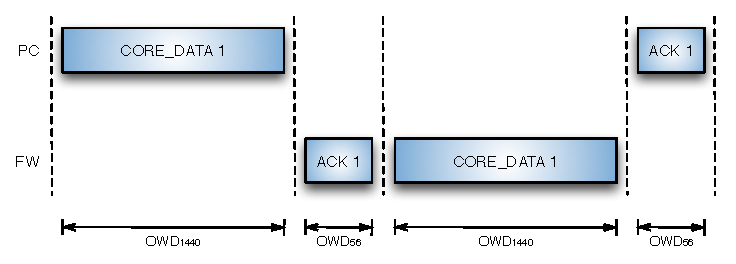
\includegraphics[scale=1,center]{Diagrams/Single-time.pdf}
  \caption{Single-Port Timing Diagram}\label{fig:singleport}
\end{figure}

Figure \ref{fig:dualport} shows the calculation of the practical upper bound for a two-port FaceWorks system. Two simultaneously working ports can send and receive back two CORE\_DATA packets in approximately 2.424 ms. The blue color represents the first port, and the red color the second port.

\begin{figure}[h]
  \centering
      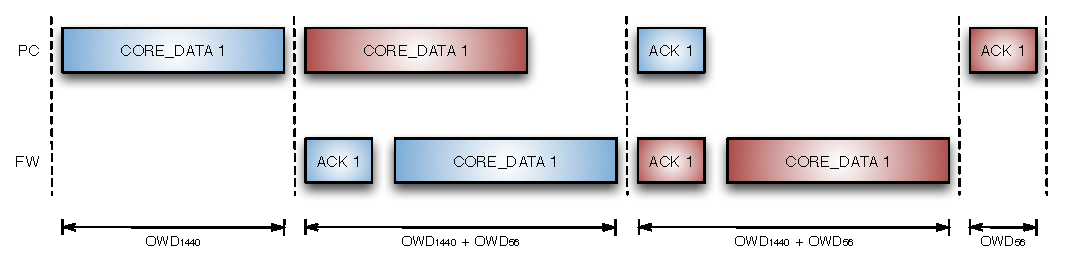
\includegraphics[scale=1,center]{Diagrams/Dual-time.pdf}
  \caption{Two-Port Timing Diagram}\label{fig:dualport}
\end{figure}


\begin{table}[h]
\centering
\caption{Throughput Model}
\label{table:Latency Model Throughput}
\begin{tabular}{c c c}
\hlinew{0.08cm}
\cellformatrG{}&\cellformatlrG{}&\cellformatlG{}\\
\cellformatrG{\multirow{-2}{*}{\centering }}&
\cellformatlrG{\multirow{-2}{2cm}{\centering Throughput}}&
\cellformatlG{\multirow{-2}{2cm}{\centering Utilization}}
\\
\hlinew{0.04cm}
\cellformatrW{Single Port} & \cellformatlrW{13.55 Mbps} & \cellformatlW{7.11\%}\\
\hlinew{0.04cm}
\cellformatrW{Dual Port} & \cellformatlrW{19.00 Mbps} & \cellformatlW{10\%}\\
\hlinew{0.08cm}
\end{tabular}
\end{table}

Converting lower bound delays to upper bound throughput yields the upper bound throughput results shown in Table \ref{table:Latency Model Throughput}. These results are considerably lower than the switch limits shown in Table \ref{table:TL-WR841N 10/100 Mb Maximum Raw Throughput}. This is made clear by column Utilization in the table, which shows the obtained throughput divided by the maximum possible throughput.  The explanation for the low utilization rate lies, firstly, in the system latency, and secondly, in the inter packet dependency between the CORE\_DATA packets and the ACK packets.

These results show that the handshaking has a dramatic effect on a single-port FaceWorks, as the next packet can only be sent after the acknowledge for the previous packet is received. The model predicts only about 14 Mbps of effective throughput using a single port.

The situation improves considerably when the second port is added, since a packet for the second port
can be sent without waiting for the acknowledge of the packet sent to the first port. The model
predicts 19 Mbps of effective throughput, which is close to the 21 Mbps limit obtained without handshaking.


\section{FaceWorks Sustained Throughput}

For the sustained\footnote{In networking the term {\it sustained} is used for results obtained by averaging over long periods of time.} throughput measurement, the previously benchmarked TP-Link TL-WR841N 10/100 Mbps switch has been used to interconnect the notebook and the FPGA board containing the FaceWorks core. In the FPGA, the CW-link RX-TX loopback shown in Figure \ref{fig:CW-LoopBack} was in place, so that the tests could be done using FaceWorks alone. Table \ref{table:FaceWorks Throughput Results} summarizes the results obtained.

\begin{table}[h]
\centering
\caption{FaceWorks Throughput Results}
\label{table:FaceWorks Throughput Results}
\begin{tabular}{c c c c}
\hlinew{0.08cm}
\cellformatrG{}&\cellformatlrG{}&\cellformatlrG{}&\cellformatlG{}\\
\cellformatrG{\multirow{-2}{*}{\centering }} &
\cellformatlrG{\multirow{-2}{2cm}{\centering Single Port}}&
\cellformatlrG{\multirow{-2}{1.8cm}{\centering Dual Port}}&
\cellformatlG{\multirow{-2}{1.8cm}{\centering Gain}}
\\
\hlinew{0.04cm}

\cellformatrW{Original FaceWorks} & \cellformatlrW{9.86 Mbps} & \cellformatlrW{-} & \cellformatlW{-}\\
\cellformatrW{Current FaceWorks} & \cellformatlrW{11.02 Mbps} & \cellformatlrW{14.71 Mbps} & \cellformatlW{33\%}\\
\cellformatrW{Verilator Model } & \cellformatlrW{42.27 Mbps} & \cellformatlrW{79.59 Mbps}& \cellformatlW{88\%}\\
\hlinew{0.08cm}
\multicolumn{4}{c}{\vspace*{-0.3cm}}\\

\end{tabular}
\end{table}


Both the original and new FaceWorks implementations have been tested using the Face-Test application. 
The new version is significantly faster than the original FaceWorks implementation in VHDL. Since the algorithms are the same, the suspicion is that the previous version may have been dropping packets, due to the presence of problems detected by the Verilator linter, which have been fixed in this new and cleaned up Verilog version. Specifically, the original code had a few combinatorial loops which may cause occasional packet losses.

The two-port FaceWorks core has been tested using two Face-Test applications, one for each UDP port. As can be seen, the two-port FaceWorks makes a better use of the available bandwidth when compared to the single-port implementation, as predicted by the throughput model of section \ref{sec:upperbound}.

Using the cycle accurate Verilator simulator, about 42 Mbps for a single-port core and 80 Mbps for a two-port core have been obtained.  Note that, in hardware simulation only, all latencies are zero (network, switch, host and \ac{OS}), except for the FaceWorks and the MAC protocol small hardware latencies. This clearly demonstrates the dramatic effect of system latency on the board measurements reported before.

The values obtained by the current FaceWorks implementation are compared with the values predicted by the throughput model in Table \ref{table:Faceworks Throughput Comparision}. The deviations can be explained by the added latency introduced by the host computer and its operating system. The two-port model performed relatively worse than the single-port model, which can be attributed to the fact that the former requires two Face-Test applications running simultaneously and competing for a shared network interface.

\begin{table}[h]
\centering
\caption{Measured vs. Modeled Throughput}
\label{table:Faceworks Throughput Comparision}
\begin{tabular}{c c c c}
\hlinew{0.08cm}
\cellformatrG{}&\cellformatlrG{}&\cellformatlrG{}&\cellformatlG{}\\
\cellformatrG{\multirow{-2}{*}{\centering }} &
\cellformatlrG{\multirow{-2}{2cm}{\centering Measured}}&
\cellformatlrG{\multirow{-2}{1.8cm}{\centering Model}}&
\cellformatlG{\multirow{-2}{1.8cm}{\centering Deviation}}
\\
\hlinew{0.04cm}

\cellformatrW{Single Port} & \cellformatlrW{11.02 Mbps} & \cellformatlrW{13.55 Mbps} & \cellformatlW{19\%}\\
\cellformatrW{Dual Port} & \cellformatlrW{14.71 Mbps} & \cellformatlrW{19.00 Mbps} & \cellformatlW{23\%}\\
\hlinew{0.08cm}
\multicolumn{4}{c}{\vspace*{-0.3cm}}\\

\end{tabular}
\end{table}
 

% %%%%%%%%%%%%%%%%%%%%%%%%%%%%%%%%%%%%%%%%%%%%%%%%%%%%%%%%%%%%%%%%%%%%%%
% Conclusion
% %%%%%%%%%%%%%%%%%%%%%%%%%%%%%%%%%%%%%%%%%%%%%%%%%%%%%%%%%%%%%%%%%%%%%%
\fancychapter{Conclusion}

\section{Summary}

The design of a new multiple port FaceWorks architecture is the main objective of this work, which has been fully accomplished, including its verification and experimental characterization. 

FaceWorks is a technology used to test and debug IP cores inside a chip by connecting this chip to an Ethernet network and conducting the tests from a regular \ac{PC}. FaceWorks is a patented and proprietary technology of the company Coreworks S.A. FaceWorks uses the UDP/IP protocol stack, topped by the proprietary CWDP layer used for direct interaction with the IP cores being debugged. The IP cores are connected to the FaceWorks module by means of the proprietary CW-Link interfaces.

The IP cores can be tested by test programs running on the PC. The main motivation of this work is to simplify the writing of test software, by allowing multiple threads or processes to exercise multiple IP cores simultaneously using two distinct UDP ports.

The design consisted of extending the FaceWorks hardware to support two ports, and writing a software application to exercise the two ports.

In the hardware implementation, the UDP and CWDP modules have been modified to work with two ports. The number of CW-Link interfaces has been duplicated, in order to keep the same number of debug interfaces per UDP port. Originally FaceWorks was written in the \ac{VHDL} language. In this work the code has been  rewritten in Verilog to allow the new developments to be done also in Verilog. Besides being a lot more common in the industry, the use of Verilog is mandatory to be able to use the Verilator simulator, a key tool which made possible the completion of this project in time.

In the software implementation, a test application (Face-Test) has been developed to send and receive test data to the device under test. This application communicates with the target using sockets, which is useful because it can stimulate both the actual hardware or a simulator. 

For verification a cutting-edge approach has been used. Instead of using a standard Verilog testbench and simulator, the Verilator simulator has been used to create a SystemC model of the FaceWorks design, which has been embedded in a C++ testbench. The testbench communicates with the Face-Test application via sockets and drives the FaceWorks SystemC model. This solves the classical problem of integrating software and hardware in a simulation environment. Other advantages of using Verilator are the detailed linting it effects on the Verilog code (due to the fact that it only supports synthesizable code), the exhaustive dumping of wave traces for debugging purposes, and the detailed coverage metrics it extracts from the design simulation. 

The design has been synthesized and tested in a Xilinx Spartan 6 \ac{FPGA}. The implementation proved small and fast enough for a debug core, as such cores should not take too much space in the overall system design. The implementation of the extra port is accomplished at the cost of extra resources. Nonetheless, the resulting FaceWorks \ac{ILP} core is still a small core, using only 10\% of the area of an average size FPGA such as the Spartan 6 XC6SLX45T device.

The performance of the core has been measured using the above mentioned FPGA and the Face-Test application. First the characterization of the used Ethernet switch was done to have practical upper bounds for bandwidth, instead of the nominal 100 Mbps. It has been measured that the switch introduces a 5\% penalty in the throughput compared to the nominal bandwidth.

Results obtained with the {\tt ping} application show that the factor limiting the system performance is the latency. The data is packetized and a latency penalty is incurred for each packet sent. Naturally the penalty decreases with the packet size but even for the maximum packet size allowed by the CWDP protocol (1440 bytes), the practical upper bound for aggregate throughput thus obtained is of about 21 Mbps.

With the delays obtained with the {\tt ping} application, a model to predict the throughput for Face-Test / FaceWorks transactions has been build. This model takes into account the handshaking implemented with small acknowledge packets. The handshaking has a dramatic effect on a single-port FaceWorks, as the next packet can only be sent after the acknowledge for the previous packet is received. The model predicts only about 14 Mbps of effective aggregate throughput using a single port. The situation improves considerably when the second port is added, since a packet for the second port can be sent without waiting for the acknowledge of the packet sent to the first port. The model predicts 19 Mbps of effective aggregate throughput, which is close to the 21 Mbps obtained without handshaking.

An experimental setup, using a Face-Test application sending and receiving packets to a single-port FaceWorks core equipped with a CW-Link loopback, showed that, in practice, only about 11 Mbps aggregate throughput can be obtained, compared to the 14 Mbps as predicted by the model. Another experiment, using two Face-Test applications sending and receiving packets to a two-port FaceWorks core, achieved about 15 Mbps, compared to the 19 Mbps predicted by the model. This difference can be explained by the added latency introduced by the host computer and its operating system. In an extreme situation where all latencies were zero (network, switch, host and OS), one could obtain about 42 Mbps for a single-port core and 80 Mbps for a two-port core; this result has been obtained using just the cycle accurate Verilator model.


\section{Future work}

To improve the FaceWorks throughput one obvious solution is upgrading it to use a 1 Gbps PHY chip. This would allow for a lower latency because of a higher transmission rate and a higher \ac{MTU} with the use of Jumbo frames. However, implementing support for Jumbo frames would require larger amounts of on-chip \acsp{RAM}, and this could be a restriction depending on the target \ac{FPGA} device.



\subsection{Not Acknowledge}

This solution consists in not sending acknowledge packets; if some packet is lost or received out-of-order then the retransmission of that packet is requested. This solution is based on the assumption that most packets sent from the PC to FaceWorks and vice-versa will be delivered and arrive in order.

Such mode would work in the following way. The controlling host (PC) starts by registering with the FaceWorks using the command SET\_CORE\_ACCESS. This command is replied with an \ac{ACK} packet. This is necessary so the PC knows that at least the first packet has been received and that it is now controlling FaceWorks. After this, \ac{ACK} packets are disabled for CORE\_DATA packets. Instead, when the receiver detects a packet whose sequence number is not $n+1$, where n is the sequence number of the previous packet, it emits a \ac{NACK} requesting the retransmission of the lost packet n+1.

\begin{figure}[h]
\centering
\subfigure[Recovery from a lost CORE\_DATA]{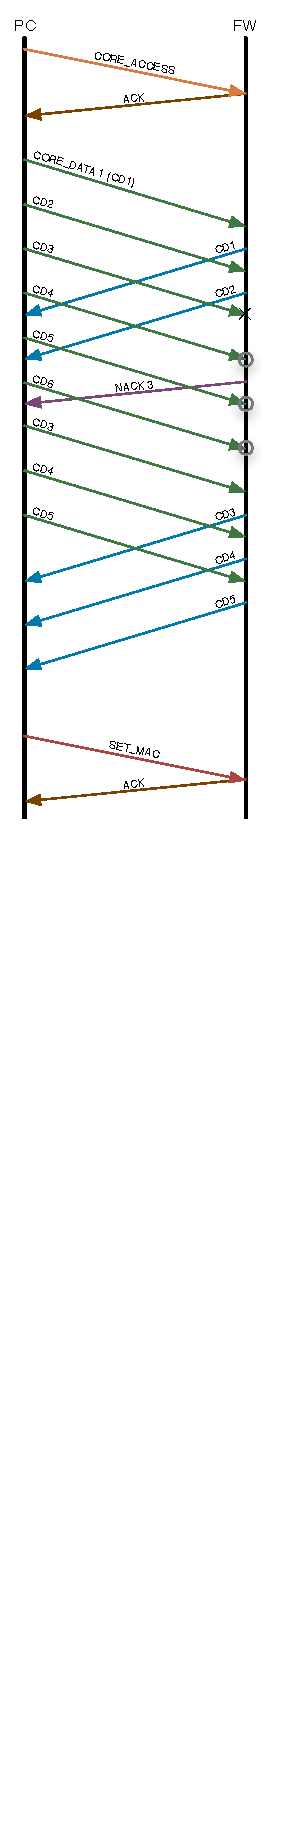
\includegraphics[scale=1.1]{Diagrams/NAC-lost.pdf}\label{fig:nacklost}}
\hspace*{2cm}
\subfigure[Recovery from a delivered out-of-order CORE\_DATA]{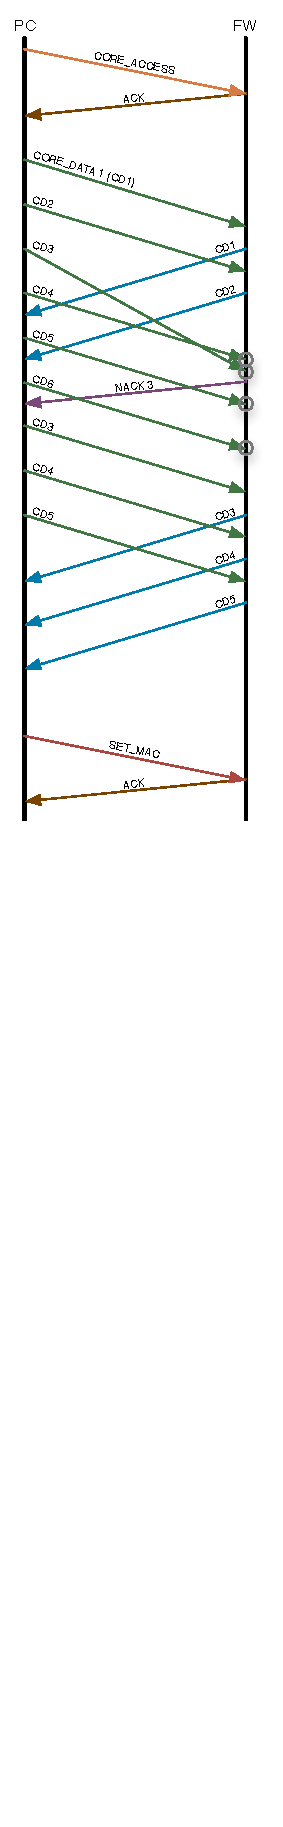
\includegraphics[scale=1.1]{Diagrams/NAC-OutOfOrder.pdf}\label{fig:nacoutoforder}}\\
\caption{Packet Loss Example Recoveries using NACK's}
\label{fig:NACK-EX}
\end{figure}

Figure \ref{fig:nacklost} shows an example transfer from the PC to FaceWorks, where packet 3 is lost. After receiving packet 4 and dropping it, FaceWorks sends a (\ac{NACK} packet for packet 3 to the PC. All subsequent packets are dropped until packet 3 is received. When packet 3 is received, the transmission resumes.

Figure \ref{fig:nacoutoforder} shows an example transfer from the PC to FaceWorks where packet 4 is delivered before packet 3. The same recovery procedure is performed as described previously.

However, the NACK solution requires a more complex software application to control the packet transmission rate, since the receipt of too many NACK packets may signal the presence of network congestion. In this case the rate of transmission should be lowered to avoid congestion. Reversely, the transmission rate can be augmented if the incidence of NACK packets is not increased.


\clearpage

\subsection{A UDP/CWDP Cycle Accurate Simulator}

The solution proposed previously for the FaceWorks simulator was designed to debug FaceWorks core itself. To debug an \ac{ILP} core having a CW-Link interface, one could simply {\it verilate} it together with FaceWorks. However, if the objective is to the debug the \ac{ILP} core only, simulating FaceWorks may be an unnecessary burden. A simpler alternative is presented in Figure \ref{fig:udpserver}. It consists in replacing the full FaceWorks model with a simple UDP/CWDP server in the C/C++ testbench.


\begin{figure}[h]
  \centering
      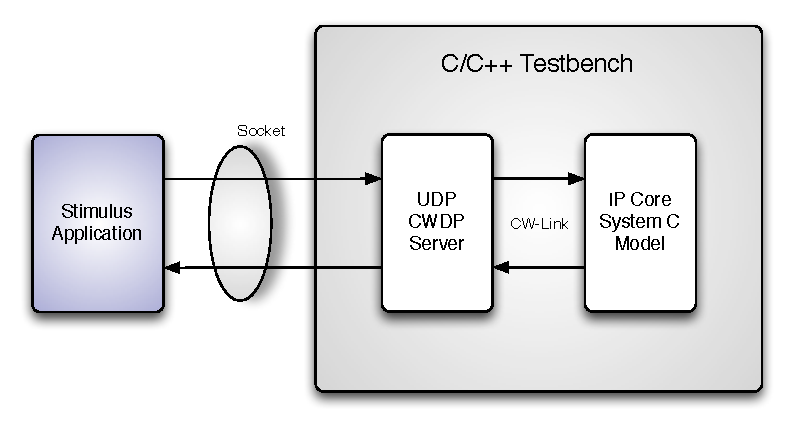
\includegraphics[scale=1,center]{Diagrams/Simp-Diag.pdf}
  \caption{A \ac{UDP}/\ac{CWDP} Cycle Accurate Simulator}\label{fig:udpserver}
\end{figure}

The UDP/CWDP server interacts with the \ac{ILP} core model using CW-Link interfaces. Test applications like Face-Test can be written in any language as long as they use network sockets for communication and implement the \ac{CWDP} protocol. These test application can later be reused to test the same \ac{ILP} core in a chip that contains the FaceWorks core. Finally, the major advantage of this approach is the fact that the simulation of the \ac{ILP} core becomes simpler and faster because the FaceWorks model is not being simulated.

% Ensure that the next chapter starts in a odd page
\cleardoublepage


% Add the Bibliography to the PDF table of contents (not the document table of contents)
\pdfbookmark[0]{Bibliography}{bib}
% The bibliography style sheet
 \bibliographystyle{IEEEtran}
 
%\bibliographystyle{apalike}
% \bibliographystyle{unsorted}
% The BiBTeX file
\bibliography{biblio}
\cleardoublepage

\appendix
% %%%%%%%%%%%%%%%%%%%%%%%%%%%%%%%%%%%%%%%%%%%%%%%%%%%%%%%%%%%%%%%%%%%%%%
% First appendix
% %%%%%%%%%%%%%%%%%%%%%%%%%%%%%%%%%%%%%%%%%%%%%%%%%%%%%%%%%%%%%%%%%%%%%%
\fancychapter{Appendix A GTKwave}
\label{Appendix A}
\begin{figure}[t]
  \centering
      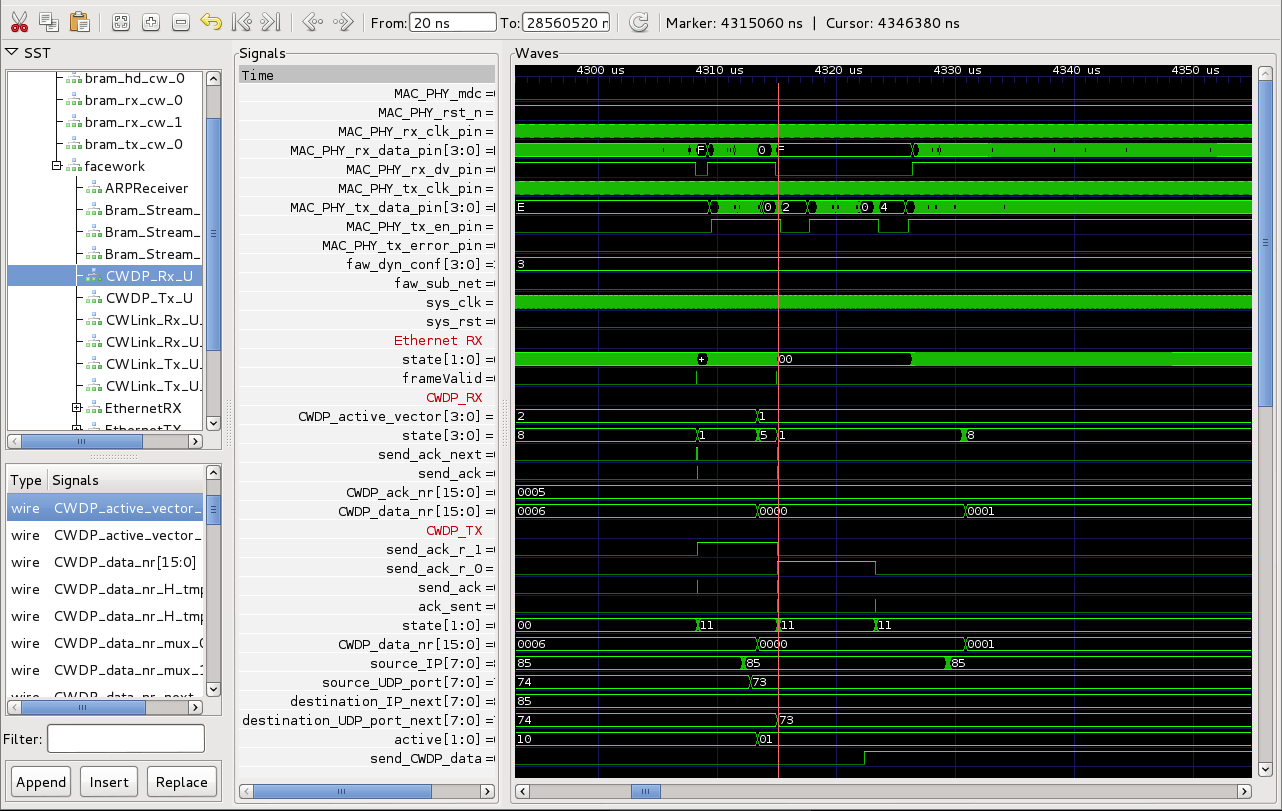
\includegraphics[scale=0.50,angle =-90 ]{Diagrams/GTKwave.png}
  \caption{A GTKwave Screenshot Showing FaceWorks Signals}
\end{figure}

\end{document}
